\documentclass[12pt,letter]{article}\usepackage[]{graphicx}\usepackage[]{color}
%% maxwidth is the original width if it is less than linewidth
%% otherwise use linewidth (to make sure the graphics do not exceed the margin)
\makeatletter
\def\maxwidth{ %
  \ifdim\Gin@nat@width>\linewidth
    \linewidth
  \else
    \Gin@nat@width
  \fi
}
\makeatother

\definecolor{fgcolor}{rgb}{0.345, 0.345, 0.345}
\newcommand{\hlnum}[1]{\textcolor[rgb]{0.686,0.059,0.569}{#1}}%
\newcommand{\hlstr}[1]{\textcolor[rgb]{0.192,0.494,0.8}{#1}}%
\newcommand{\hlcom}[1]{\textcolor[rgb]{0.678,0.584,0.686}{\textit{#1}}}%
\newcommand{\hlopt}[1]{\textcolor[rgb]{0,0,0}{#1}}%
\newcommand{\hlstd}[1]{\textcolor[rgb]{0.345,0.345,0.345}{#1}}%
\newcommand{\hlkwa}[1]{\textcolor[rgb]{0.161,0.373,0.58}{\textbf{#1}}}%
\newcommand{\hlkwb}[1]{\textcolor[rgb]{0.69,0.353,0.396}{#1}}%
\newcommand{\hlkwc}[1]{\textcolor[rgb]{0.333,0.667,0.333}{#1}}%
\newcommand{\hlkwd}[1]{\textcolor[rgb]{0.737,0.353,0.396}{\textbf{#1}}}%
\let\hlipl\hlkwb

\usepackage{framed}
\makeatletter
\newenvironment{kframe}{%
 \def\at@end@of@kframe{}%
 \ifinner\ifhmode%
  \def\at@end@of@kframe{\end{minipage}}%
  \begin{minipage}{\columnwidth}%
 \fi\fi%
 \def\FrameCommand##1{\hskip\@totalleftmargin \hskip-\fboxsep
 \colorbox{shadecolor}{##1}\hskip-\fboxsep
     % There is no \\@totalrightmargin, so:
     \hskip-\linewidth \hskip-\@totalleftmargin \hskip\columnwidth}%
 \MakeFramed {\advance\hsize-\width
   \@totalleftmargin\z@ \linewidth\hsize
   \@setminipage}}%
 {\par\unskip\endMakeFramed%
 \at@end@of@kframe}
\makeatother

\definecolor{shadecolor}{rgb}{.97, .97, .97}
\definecolor{messagecolor}{rgb}{0, 0, 0}
\definecolor{warningcolor}{rgb}{1, 0, 1}
\definecolor{errorcolor}{rgb}{1, 0, 0}
\newenvironment{knitrout}{}{} % an empty environment to be redefined in TeX

\usepackage{alltt}    

%########################################################################################  
%            						PACKAGES
%########################################################################################

\usepackage{authblk} % for author affiliations
\usepackage{float} % for H in figures and tables
\usepackage{amsmath,amsthm,amssymb,bbm,mathrsfs,mathtools,xfrac} %math stuff

\usepackage[sort]{natbib}   % bibliography omit 'round' option if you prefer square brackets
\usepackage{placeins} % for \FloatBarrier
\usepackage[pagebackref=true,bookmarks]{hyperref}
\hypersetup{
	unicode=false,          
	pdftoolbar=true,        
	pdfmenubar=true,        
	pdffitwindow=false,     % window fit to page when opened
	pdfstartview={FitH},    % fits the width of the page to the window
	pdftitle={Sparse Additive Interaction Learning},    % title
	pdfauthor={Sahir Rai Bhatnagar},     % author
	pdfsubject={sail manuscript},   % subject of the document
	pdfcreator={Sahir Rai Bhatnagar},   % creator of the document
	pdfproducer={Sahir Rai Bhatnagar}, % producer of the document
	pdfkeywords={}, % list of keywords
	pdfnewwindow=true,      % links in new window
	colorlinks=true,       % false: boxed links; true: colored links
	linkcolor=red,          % color of internal links (change box color with linkbordercolor)
	citecolor=blue,        % color of links to bibliography
	filecolor=black,      % color of file links
	urlcolor=cyan           % color of external links
}
\usepackage[utf8]{inputenc} % for french accents
\usepackage[T1]{fontenc} % for french accents
\usepackage{ctable} % load after tikz. used for tables
\usepackage{pifont}% http://ctan.org/pkg/pifont
\newcommand{\cmark}{\ding{51}}%
\newcommand{\xmark}{\ding{55}}%
\def\widebar#1{\overline{#1}}
\usepackage{array}
\newcolumntype{L}{>{\centering\arraybackslash}m{3cm}} % used for text wrapping in ctable
\usepackage{color, colortbl, xcolor, comment}
\usepackage{subfig}
\usepackage{tcolorbox} % for box around text
%\usepackage[ruled,vlined,linesnumbered,noresetcount]{algorithm2e}
%\usepackage[ruled,vlined,noresetcount]{algorithm2e}
\usepackage{algorithm}
\usepackage[noend]{algpseudocode}
\algrenewcommand\textproc{}% Used to be \textsc
\algdef{SE}[SUBALG]{Indent}{EndIndent}{}{\algorithmicend\ }%
\algtext*{Indent}
\algtext*{EndIndent}
%\usepackage[american]{babel}
%\let\tnote\relax

%\usepackage{csquotes}



%\usepackage[style=apa,sortcites=true,sorting=nyt,backend=biber]{biblatex}
%\usepackage{epstopdf}

%\usepackage{tabulary}
%\usepackage{siunitx}
%\sisetup{output-exponent-marker=\ensuremath{\mathrm{e}}}
%\AtBeginEnvironment{tabulary}{\onehalfspacing}
%\usepackage{multirow}
%\usepackage{ctable} % NEED TO LOAD CTABLE AFTER TIKZ FOR SOME REASON
%\usepackage{array}
%\newcolumntype{L}{>{\centering\arraybackslash}m{3cm}} % used for text wrapping in ctable
%\usepackage{enumitem}
% These packages are all incorporated in the memoir class to one degree or another...

%########################################################################################  
%            						CUSTOM COMMANDS
%########################################################################################

\newcommand{\sail}{\texttt{sail }}
\newcommand{\tm}[1]{\textrm{{#1}}}
\newcommand{\bx}{\textbf{\emph{x}}}
\newcommand{\by}{\textbf{\emph{y}}}
\newcommand{\bX}{\textbf{\emph{X}}}
\newcommand{\bW}{\textbf{\emph{W}}}
\newcommand{\bY}{\textbf{\emph{Y}}}
\newcommand{\bD}{\textbf{\emph{D}}}
\newcommand{\bXtilde}{\widetilde{\bX}}
\newcommand{\bYtilde}{\widetilde{\bY}}
\newcommand{\bDtilde}{\widetilde{\bD}}
\newcommand{\Xtilde}{\widetilde{X}}
\newcommand{\Ytilde}{\widetilde{Y}}
\newcommand{\Dtilde}{\widetilde{D}}
\newcommand{\bu}{\textbf{u}}
\newcommand{\bU}{\textbf{\emph{U}}}
\newcommand{\bV}{\textbf{\emph{V}}}
\newcommand{\bE}{\textbf{\emph{E}}}
\newcommand{\bb}{\textbf{\emph{b}}}
\newcommand{\bI}{\textbf{\emph{I}}}
\newcommand{\be}{\boldsymbol{\varepsilon}}
\newcommand{\bSigma}{\boldsymbol{\Sigma}}
\newcommand{\bLambda}{\boldsymbol{\Lambda}}
\newcommand{\bTheta}{\boldsymbol{\Theta}}
\newcommand{\balpha}{\boldsymbol{\alpha}}
%\newcommand{\ltwonorm}[1]{\lVert #1 \rVert}
\newcommand{\mb}[1]{\mathbf{#1}}
\newcommand {\bs}{\boldsymbol}
%\newcommand{\norm}[1]{\left\Vert #1 \right\Vert} 
\newcommand{\xf}{\mathcal{X}}
\newcommand{\pfrac}[2]{\left( \frac{#1}{#2}\right)}
\newcommand{\e}{{\mathsf E}}
\newcommand{\bt}{\boldsymbol{\theta}}
\newcommand{\bmu}{\boldsymbol{\mu}}
\newcommand{\bbeta}{\boldsymbol{\beta}}
\newcommand{\btheta}{\boldsymbol{\theta}}
\newcommand{\bPhi}{\boldsymbol{\Phi}}
\newcommand{\bPsi}{\boldsymbol{\Psi}}
\DeclareMathOperator*{\argmin}{arg\,min}
\DeclareMathOperator*{\argmax}{arg\,max}
\DeclareMathOperator{\diag}{diag} % operator and subscript

\DeclarePairedDelimiter\abs{\lvert}{\rvert}%
\DeclarePairedDelimiter\norm{\lVert}{\rVert}%

% Swap the definition of \abs* and \norm*, so that \abs
% and \norm resizes the size of the brackets, and the 
% starred version does not.
\makeatletter
\let\oldabs\abs
\def\abs{\@ifstar{\oldabs}{\oldabs*}}
%
\let\oldnorm\norm
\def\norm{\@ifstar{\oldnorm}{\oldnorm*}}
\makeatother

%########################################################################################  
%            						FANCY HEADER STUFF
%######################################################################################## 
\usepackage{lastpage}
\usepackage{fancyhdr}
\cfoot{\thepage}
\lhead[\leftmark]{}
\rhead[]{\leftmark}
\makeatletter
\makeatother
\lfoot{} \cfoot{ } \rfoot{{\small{\em Page \thepage \ of \pageref{LastPage}}}}


%########################################################################################  
%            						SPACING
%######################################################################################## 

\usepackage[parfill]{parskip} % Activate to begin paragraphs with an empty line rather than an indent
%\usepackage[left=.1in,right=.1in,top=.1in,bottom=.1in]{geometry}
\usepackage[margin=1in]{geometry}
\usepackage{setspace}
\doublespacing

%########################################################################################  
%            						TITLE and AUTHORS
%########################################################################################

\title{Sparse Additive Interaction Learning}
%\author{SRB}

\author[1,2]{Sahir R Bhatnagar}
%\author[3]{Karim Oualkacha}
\author[4]{Yi Yang}
\author[1,2,5]{\mbox{Celia MT Greenwood}}
\affil[1]{Department of Epidemiology, Biostatistics and Occupational Health, McGill University}
\affil[2]{Lady Davis Institute, Jewish General Hospital, Montr\'{e}al, QC}
%\affil[3]{Département de Mathématiques, Université de Québec À Montréal}
\affil[4]{Department of Mathematics and Statistics, McGill University}
\affil[5]{Departments of Oncology and Human Genetics, McGill University}

%########################################################################################  
%            						START OF DOCUMENT
%########################################################################################
\IfFileExists{upquote.sty}{\usepackage{upquote}}{}
\begin{document}







\maketitle
\pagestyle{fancy}


\maketitle
\section{Introduction}

Computational approaches to variable selection have become increasingly important with the advent of high-throughput technologies in genomics and brain imaging studies, where the data has become massive, yet where it is believed that the number of truly important variables is small relative to the total number of variables. Although many approaches have been developed for main effects, there are several applications where interaction models can reflect biological phenomena and improve statistical power.  For example, genome wide association studies (GWAS) have been unable to explain a large proportion of heritability (the variance in phenotype attributable to genetic variants) and it has been suggested that this missing heritability may in part be due to gene-environment interactions~\citep{manolio2009finding}.  Furthermore, diseases are now thought to be the result of entire biological networks whose states are affected by environmental factors, and these systemic changes can induce or eliminate strong correlations between elements in a network. Therefore, we propose a multivariate penalization procedure for detecting interactions between high dimensional data ($p >> n$) and an environmental factor, where the effect of this environmental factor on the high dimensional data is widespread and plays a role in predicting the response. Our approach improves on existing procedures for detecting such interactions in three ways; 1) it automatically enforces the strong heredity property, i.e., an interaction term can only be included in the model if the corresponding main effects are in the model 2) it reduces the dimensionality of the problem and leverages the high correlations by transforming the input feature space using network connectivity measures and 3) it leads to interpretable models which are biologically meaningful. This thesis is motivated by three studies; one that looks at the impact of maternal care on child development, another that characterizes normal brain development as a function of intelligence scores and one that looks at the long-lasting effects of diet in subsequent generations.


%Diseases are now thought to be the result of changes in entire biological networks whose states are affected by a complex interaction of genetic and environmental factors. In general, power to estimate interactions is low, the number of possible interactions could be enormous and their effects may be non-linear. Existing approaches such as the lasso might keep an interaction but remove a main effect, which is problematic for interpretation.




We consider a regression model for an outcome variable $Y=(Y_1, \ldots, Y_n)$ where $n$ is the number of subjects. 
Let $E=(E_1, \ldots, E_n)$ be a binary or continuous environment vector and \mbox{$\bX = (X_{1}, \ldots, X_{n})^\top$} be the $n \times p$ matrix of high-dimensional data where $X_i = (X_{i1}, \ldots,X_{ij}, \ldots,  X_{ip}) $, and $\bs{\varepsilon} = (\varepsilon_1, \ldots, \varepsilon_n)$ a vector of errors. 
Consider the regression model with main effects and their interactions with $E$:
\begin{equation}  
g(\bmu) =  \beta_0 + \sum_{j=1}^p \beta_j X_{j} + \beta_E E + \sum_{j=1}^p \alpha_j E X_j \label{eq:linpred1.1} , %\qquad i=1, \ldots, n ,
\end{equation}
where $g(\cdot)$ is a known link function, $\bmu = \e\left[Y|\bX, E, \bbeta,\balpha\right]$, and $\beta_0,\beta_j,\beta_E,\alpha_j$ are the true unknown model parameters for $j=1, \ldots, p$. 

Due to the large number of parameters to estimate with respect to the number of observations, one commonly-used approach is to shrink the regression coefficients by placing a constraint on the values of $\bbeta$ and $\boldsymbol{\alpha}$. For example, the LASSO~\citep{tibshirani1996regression} penalizes the squared loss of the data with the \mbox{$L_1$-norm} of the regression coefficients resulting in a method that performs both model selection and estimation. A natural extension of the LASSO to the interaction model~\eqref{eq:linpred1.1} is given by:
\begin{equation}
\argmin_{\beta_0, \bbeta, \boldsymbol{\alpha} }  \frac{1}{2} \norm{Y - g(\bmu)}^2 + \lambda \left( \norm{\bbeta}_1 + \norm{\balpha}_1    \right) \label{eq:lassolikelihood}
\end{equation}
where $\norm{Y - g(\bmu)}^2 = \sum_i (y_i - g(\mu_i))^2$, $\norm{\bbeta}_1 = \sum_j | \beta_j  |$, $\norm{\balpha}_1 = \sum_j | \alpha_j  |$ and $\lambda \geq 0$ is a data driven tuning parameter that can set some of the coefficients to zero when sufficiently large. 

However, since no constraint is placed on the structure of the model in~\ref{eq:lassolikelihood}, it is possible that the estimated main effects are zero while the interaction term is not. This has motivated methods that produce structured sparsity~\citep{bach2012structured}. For example, Bien \textit{et al.}~\citep{bien2013lasso} propose a strong hierarchical lasso which forces the main effects to be included if the interaction term is non-zero. However this method and related ones are restricted to all pairwise interactions between $p$ measured variables. Here were concern ouself with methods that impose a strong hierarchy in the context of gene environment interactions. We are interested in imposing the strong heredity principle~\citep{chipman1996bayesian}: 
\begin{equation}
\hat{\alpha}_{j} \neq 0 \qquad \Rightarrow \qquad \hat{\beta}_j \neq 0 \qquad \tm{and} \qquad \hat{\beta}_E \neq 0   \label{eq:heredity}
\end{equation}
In words, the interaction term will only have a non-zero estimate if its corresponding main effects are estimated to be non-zero. One benefit brought by hierarchy is that the number of measured variables can be reduced, referred to as practical sparsity~\citep{she2014group,bien2013lasso}. For example, a model involving $X_1, E, X_1 \cdot E$ is more parsimonious than a model involving $X_1, E, X_2 \cdot E$, because in the first model a researcher would only have to measure two variables compared to three in the second model. In order to address these issues, we propose to extend the model of~\citep{choi2010variable} to simultaneously perform variable selection, estimation and impose the strong heredity principle in the context of high dimensional interactions with the environment (HD$\times E$). To do so, we follow Choi and reparametrize the coefficients for the interaction terms as $\alpha_{j} = \gamma_{j} \beta_j \beta_E$. Plugging this into~\eqref{eq:linpred1.1}:
\begin{align}
g(\bmu)  = & \beta_0 + \sum_{j=1}^p \beta_j X_{j} + \beta_E E + \sum_{j=1}^p \gamma_{j} \beta_j \beta_E E X_j     \label{eq:linpred2}
\end{align}
This reparametrization directly enforces the strong heredity principle~\eqref{eq:heredity}, i.e., if either main effect estimates are 0, then $\hat{\alpha}_{j}$ will be zero and a non-zero interaction coefficient implies non-zero $\hat{\beta}_j$ and $\hat{\beta}_E$. To perform variable selection in this new parametrization, we follow~\cite{choi2010variable} and penalize $\bs{\gamma} = \left(\gamma_{1}, \ldots, \gamma_{p}\right)$ instead of penalizing $\balpha$ as in~\eqref{eq:lassolikelihood}, leading to the following penalized least squares criterion:
\begin{equation}
\argmin_{\beta_0, \bbeta, \bs{\gamma} }  \frac{1}{2} \norm{Y - g(\bmu)}^2 + \lambda_\beta \sum_{j=1}^{p}w_j \abs{\beta_j} + \lambda_\gamma \sum_{j=1}^{p} w_{jE} \abs{\gamma_{jE}} \label{eq:lassolikelihood2}
\end{equation} 
where $g(\bmu)$ is from~\eqref{eq:linpred2}, $\lambda_\beta$ and $\lambda_\gamma$ are tuning parameters and $\mb{w} = \left(w_{1}, \ldots, w_q, w_{1E}, \ldots, w_{qE}\right)$ are prespecified adaptive weights. The $\lambda_\beta$ tuning parameter controls the amount of shrinkage applied to the main effects, while $\lambda_\gamma$ controls the interaction estimates and allows for the possibility of excluding the interaction term from the model even if the corresponding main effects are non-zero. The adaptive weights serve as a way of allowing parameters to be penalized differently. Furthermore, adaptive weighting~\citep{zou2006adaptive} has been shown to construct oracle procedures~\citep{fan2001variable}, i.e., asymptotically, it performs as well as if the true model were given in advance. The oracle property is achieved when the weights are a function of any root-$n$ consistent estimator of the true parameters e.g. maximum likelihood (MLE) or ridge regression estimates. It can be shown that the procedure in~\eqref{eq:lassolikelihood2} asymptotically possesses the oracle property~\citep{choi2010variable}, even when the number of parameters tends to $\infty$ as the sample size increases, if the weights are chosen such that
\begin{equation}
w_j = \left | \frac{1}{\hat{\beta}_j} \right|, \quad w_{jE} = \left | \frac{\hat{\beta}_j \hat{\beta}_E}{\hat{\alpha}_{jE}} \right| \quad \tm{ for }j=1, \ldots, q   \label{eq:weights}
\end{equation}
where $\hat{\beta}_j$ and $\hat{\alpha}_{j}$ are the MLEs, from~\eqref{eq:linpred1.1} or the ridge regression estimates when $p > n$. The rationale behind the data-dependent $\hat{\bs{w}}$ is that as the sample size grows, the weights for the truly zero predictors go to $\infty$ (which translates to a large penalty), whereas the weights for the truly non-zero predictors converge to a finite constant~\citep{zou2006adaptive}. 


\subsection{Toy example}

We begin with a toy example to better illustrate our method. We sample $p=20$ covariates independently from a $N(0,1)$ truncated to the interval [0,1] and sample size $N=100$. We generated data from the model
\begin{equation}
	Y = f_1(X_1) + f_2(X_2) + 1.75 E + 1.5 E \cdot f_2(X_2) + \varepsilon
\end{equation}
where $f_1(x) = -3x$, $f_2(x) = 2(2x-1)^3$ and the error term $\varepsilon$ is generated from a normal distribution with variance chosen such that the signal-to-noise ratio (SNR) is 2. We run the \sail method with cubic b-splines and 10-fold CV to choose the optimal value of $\lambda$. Default values were used for all other arguments. We plot the solution path for both main effects and interactions in Figure~\ref{fig:toy-solution-path} and the estimated functions $\hat{f}_1$ and $\hat{f}_2$ in Figure~\ref{fig:toy-effects}.








\subsection{Existing Literature}

\ctable[pos=h!,doinside=\footnotesize]{lcc}{
}{
\FL
Type      & Model   & Software \ML
\multicolumn{1}{m{1cm}}{Linear}    & \multicolumn{1}{m{6cm}}{\texttt{CAP} (Zhao et al. 2009, \emph{Ann. Stat})}        &   \xmark    \\
& \multicolumn{1}{m{8cm}}{\texttt{SHIM} (Choi et al. 2009, \emph{JASA})}        &   \xmark    \\
& \multicolumn{1}{m{8cm}}{\texttt{hiernet} (Bien et al. 2013, \emph{Ann. Stat})}        &   \texttt{hierNet(x, y)}    \\
& \multicolumn{1}{m{8cm}}{\texttt{GRESH} (She and Jiang 2014, \emph{JASA})}        &  \xmark     \\
& \multicolumn{1}{m{8cm}}{\texttt{FAMILY} (Haris et al. 2014, \emph{JCGS})}    &  \texttt{FAMILY(x, z, y)}   \\
& \multicolumn{1}{m{8cm}}{\texttt{glinternet} (Lim and Hastie 2015, \emph{JCGS})}    & \texttt{glinternet(x, y)}  \\			   	 	& \multicolumn{1}{m{6cm}}{\texttt{RAMP} (Hao et al. 2016, \emph{JASA})}        & \texttt{RAMP(x, y)}   \ML
\multicolumn{1}{m{1cm}}{Non-linear} 	& \multicolumn{1}{m{8cm}}{\texttt{VANISH} (Radchenko and James 2010, \emph{JASA})}        & \xmark  \\
& \multicolumn{1}{m{8cm}}{\texttt{sail} (Bhatnagar et al. 2017+)}        & \texttt{sail(x, e, y)}  \LL
}




\section{Extension to Additive Models}
Let $Y=(Y_1, \ldots, Y_n) \in \mathbb{R}^n$ be a continuous outcome variable, \mbox{$X_E=(E_1, \ldots, E_n) \in \mathbb{R}^n$} a binary or continuous environment vector, \mbox{$\bX = (X_{1}, \ldots, X_{p}) \in \mathbb{R}^{n\times p}$} a matrix of predictors, and $\varepsilon = (\varepsilon_1, \ldots, \varepsilon_n) \in \mathbb{R}^n$ a vector of i.i.d random variables with mean 0. Furthermore let $f_j: \mathbb{R} \rightarrow \mathbb{R}$ be a smoothing method for variable $X_j$ by a projection on to a set of basis functions:
\begin{equation}
	f_j(X_j) = \sum_{\ell = 1}^{m_j} \psi_{j\ell}(X_j) \beta_{j\ell} \label{eq:smooth}
\end{equation}
Here, the $\left\lbrace \psi_{j\ell} \right\rbrace_1^{m_j}$ are a family of basis functions in $X_j$~\citep{hastie2015statistical}. Let $\bPsi_j$ be the $n \times m_j$ matrix of evaluations of the $\psi_{j\ell}$ and \mbox{$\btheta_j = (\beta_{j1}, \ldots, \beta_{jm_j}) \in \mathbb{R}^{m_j}$} for $j = 1, \ldots, p$, i.e., $\btheta_j$ is a $m_j$-dimensional column vector of basis coefficients for the $j$th main effect. In this article we consider an additive interaction regression model of the form 
\begin{align}
	Y  & =  \beta_0 \cdot \boldsymbol{1} + \sum_{j=1}^p \bPsi_j \btheta_j + \beta_E X_E + \sum_{j=1}^p (X_E \circ \bPsi_j) \balpha_{j}  + \varepsilon  \label{eq:linpred}
\end{align}
\begin{comment}
Define the smoothing method for variable $X_j$ by a projection on to a set of basis functions:
\begin{equation}
f_j(\cdot) = \sum_{\ell = 1}^{p_j} \psi_{j\ell}(\cdot) \beta_{j\ell} \label{eq:smooth}
\end{equation}
Here, the $\left\lbrace \psi_{j\ell} \right\rbrace_1^{p_j}$ are a family of basis functions in $X_j$~\citep{hastie2015statistical}. Let $\bPsi_j$ be the $n \times p_j$ matrix of evaluations of the $\psi_{j\ell}$ and \mbox{$\theta_j = (\beta_{j1}, \ldots, \beta_{jp_j})$} for $j = 1, \ldots, p$. We propose to extend~\eqref{eq:linpred1.1} to the more general additive model:
\begin{align}
g(\bmu)  = & \beta_0 + \sum_{j=1}^p \bPsi_j \theta_j + \beta_E X_E + \sum_{j=1}^p \alpha_{j} X_E \bPsi_j     
\end{align}
where $g(\cdot)$ is a known link function, $\bmu = \e\left[Y|\bX, X_E, \btheta,\balpha\right]$, and $\beta_0,\theta_j,\beta_E,\alpha_j$ are the true unknown model parameters for $j=1, \ldots, p$.
\end{comment}
where $\beta_0$ is the intercept, $\beta_E$ is the coefficient for the environment variable, $\balpha_j = (\alpha_{j1}, \ldots, \alpha_{jm_j})\in \mathbb{R}^{m_j}$ are the basis coefficients for the $j$th interaction term and $(X_E \circ \bPsi_j)$ is the $n \times m_j$ matrix formed by the component-wise multiplication of the column vector $X_E$ by each column of $\bPsi_j$. To enforce the strong heredity property, we reparametrize the coefficients for the interaction terms in~\eqref{eq:linpred} as $\balpha_{j} = \gamma_{j}  \beta_E \btheta_j$:
\begin{align}
	Y  & =  \beta_0 \cdot \boldsymbol{1} + \sum_{j=1}^p \bPsi_j \btheta_j + \beta_E X_E + \sum_{j=1}^p \gamma_{j}  \beta_E (X_E \circ \bPsi_j) \btheta_j + \varepsilon   \label{eq:linpred2}
\end{align}
%where $\norm{\theta_j}_2 = \sqrt{\sum_{\ell=1}^{p_j} \beta_{j\ell}^2}$
\begin{comment}
\begin{equation}  
Y_i = \beta^*_0 + \sum_{j=1}^p f^*_j (X_{ij}) + f_E^*(E_i) + \sum_{j=1}^p f^*_{jE} (X_{ij},E_i) + \varepsilon_i \qquad i=1, \ldots, n \label{eq:linpred1.2}
\end{equation}
As in~\citep{radchenko2010variable}, we can express~\eqref{eq:linpred1.2} as 
\begin{equation}
\mb{Y} =  \sum_{j=1}^p \mb{f}^*_j + \mb{f}_E^* + \sum_{j=1}^p \mb{f}^*_{jE} + \bs{\varepsilon} \label{eq:linpred1.3}
\end{equation}
where $\mb{f}^*_j = \left(f_j^*(X_{1j}), \ldots, f_j^*(X_{nj})\right)^\top$, $\mb{f}^*_{jE} = \left(f_{jE}^*(X_{1j},X_{1E}), \ldots, f_j^*(X_{nj}, X_{nE})\right)^\top$ and \mbox{$\mb{f}_E^* = f_E^*(E_i)$}. 
We consider the candidate vectors $\left\lbrace \mb{f}_j,\mb{f}_E, \mb{f}_{jE}\right\rbrace$. The general approach for fitting~\eqref{eq:linpred1.3} is to minimize the following penalized regression criterion:
\begin{equation}
\frac{1}{2} \lvert\lvert \mb{Y} - \mb{f} \rvert\rvert^2 + P(\mb{f})
\end{equation}
where 
\begin{equation}
\mb{f} = \sum_{j=1}^p \mb{f}_j + \mb{f}_E + \sum_{j=1}^p \mb{f}_{jE}
\end{equation}
and $P(\mb{f})$ is a penalty function on $\mb{f}$
Let 
\begin{equation}
f_{jE}(X_{j}, E) = \sum_{\ell = 1}^{q_j} \phi_{j\ell}(X_j, E) \alpha_{j\ell} \label{eq:smoothinter}
\end{equation}
where the $\left\lbrace \phi_{j\ell} \right\rbrace_1^{q_j}$ are a family of basis functions in $X_j\cdot E$.

Following ~\citep{choi2010variable}, we reparametrize the coefficients for the interaction terms as $\alpha_{j\ell} = \gamma_{j\ell} \beta_{j\ell} \beta_E$. Plugging this into~\eqref{eq:smoothinter}:
\begin{equation}
f_{jE}(X_{j}, E) = \sum_{\ell = 1}^{q_j} \phi_{j\ell}(X_j, E) \gamma_{j\ell} \beta_{j\ell} \beta_E \label{eq:smoothinter2}
\end{equation}
\end{comment}
For a continuous response, we use the squared-error loss:
\begin{equation}
	\mathcal{L}(Y;\bTheta) = \frac{1}{2n}\norm{Y - \beta_0 \cdot \boldsymbol{1} - \sum_{j=1}^p \bPsi_j \btheta_j - \beta_E X_E - \sum_{j=1}^p \gamma_{j}  \beta_E (X_E \circ \bPsi_j) \btheta_j}_2^2
\end{equation}
where $\bTheta \coloneqq (\beta_0, \beta_E,\btheta_1, \ldots, \btheta_p, \gamma_1, \ldots, \gamma_p)$. 

We consider the following penalized least squares criterion for this problem:
\begin{equation}
	\argmin_{\bTheta }  \mathcal{L}(Y;\bTheta) + \lambda (1-\alpha)  \left( w_E \abs{\beta_E} + \sum_{j=1}^{p} w_j \norm{\btheta_j}_2 \right) +  \lambda\alpha \sum_{j=1}^{p} w_{jE} \abs{\gamma_{j}} \label{eq:lassolikelihood3}
\end{equation} 
where $\lambda >0$ and $\alpha \in (0,1)$ are tuning parameters and $w_E, w_j, w_{jE}$ are adaptive weights for $j=1, \ldots, p$. These weights serve as a way of allowing parameters to be penalized differently. Furthermore, adaptive weighting~\citep{zou2006adaptive} has been shown to construct oracle procedures~\citep{fan2001variable}, i.e., asymptotically, it performs as well as if the true model were given in advance. These weights are given by
\begin{equation}
	w_E = \left|   \frac{1}{\hat{\beta}_E} \right| ,\quad w_j = \frac{1}{\norm{\hat{\btheta}_j}_2} , \quad w_{jE} = \left | \frac{\hat{\beta}_E \norm{\hat{\btheta}_j}_2}{\norm{\hat{\alpha}_{j}}_2} \right| \quad \tm{ for }j=1, \ldots, p   \label{eq:weights}
\end{equation}
where $\hat{\beta}_E$, $\hat{\btheta}_j$ and $\hat{\balpha}_{j}$ are the MLEs, from~\eqref{eq:linpred} or the ridge regression estimates when $p > n$.


%\newpage

\section{Regularization Path}
The \texttt{sail} model has the form
\begin{equation}
	\hat{Y}   =  \beta_0 \cdot \boldsymbol{1} + \sum_{j=1}^p \bPsi_j \btheta_j + \beta_E X_E + \sum_{j=1}^p \gamma_{j}  \beta_E (X_E \circ \bPsi_j) \btheta_j
\end{equation}
The objective function is given by 
\begin{equation}
	Q(\bTheta) = \frac{1}{2n} \norm{Y - \hat{Y}}_2^2 + \lambda (1-\alpha)  \left( w_E \abs{\beta_E} + \sum_{j=1}^{p} w_j \norm{\btheta_j}_2 \right) +  \lambda\alpha \sum_{j=1}^{p} w_{jE} \abs{\gamma_{j}} \label{eq:objective_least-squares}
\end{equation}
Denote the $n$-dimensional residual column vector $R = Y-\hat{Y}$. The subgradient equations are given by
\begin{align}
	\frac{\partial Q}{\partial \beta_0} & = \frac{1}{n} \left( Y - \beta_0 \cdot \boldsymbol{1} - \sum_{j=1}^p \bPsi_j \btheta_j - \beta_E X_E - \sum_{j=1}^p \gamma_{j}  \beta_E (X_E \circ \bPsi_j) \btheta_j\right)^\top \boldsymbol{1}  = 0 \label{eq:sub_b0} \\
	\frac{\partial Q}{\partial \beta_E} & = -\frac{1}{n} \left(X_E + \sum_{j=1}^{p}\gamma_j (X_E \circ \bPsi_j)\btheta_j\right)^\top R  + \lambda (1-\alpha) w_E s_1 = 0 \label{eq:sub_bE}\\
	\frac{\partial Q}{\partial \btheta_j} & = -\frac{1}{n} \left(\bPsi_j + \gamma_j \beta_E (X_E \circ \bPsi_j)\right)^\top R  + \lambda (1-\alpha) w_j s_2 = \boldsymbol{0} \label{eq:sub_thetaj}\\
	\frac{\partial Q}{\partial \gamma_j} & = -\frac{1}{n} \left(\beta_E (X_E \circ \bPsi_j)\btheta_j\right)^\top R  + \lambda \alpha w_{jE} s_3 = 0 \label{eq:sub_gammaj}
\end{align}
where $s_1$ is in the subgradient of the $\ell_1$ norm:
$$
s_1 \in \begin{cases}
\textrm{sign}\left(\beta_E\right) & \tm{if  } \beta_E \neq 0\\
[-1, 1] &  \tm{if  } \beta_E = 0,\\
\end{cases}
$$
$s_2$ is in the subgradient of the $\ell_2$ norm:
$$
s_2 \in \begin{cases}
\dfrac{\btheta_j}{\norm{\btheta_j}_2} &  \tm{if  } \btheta_j \neq \boldsymbol{0}\\
u \in \mathbb{R}^{m_j}: \norm{u}_2 \leq 1 & \tm{if  } \btheta_j = \boldsymbol{0},\\
\end{cases}
$$
and $s_3$ is in the subgradient of the $\ell_1$ norm:
$$
s_3 \in \begin{cases}
\textrm{sign}\left(\gamma_j\right) & \tm{if  } \gamma_j \neq 0\\
[-1, 1] &  \tm{if  } \gamma_j = 0.\\
\end{cases}
$$
Define the partial residuals, without the $j$th predictor for $j=1, \ldots, p$, as
\[R_{(-j)} = Y - \beta_0 \cdot \boldsymbol{1} - \sum_{\ell \neq j} \bPsi_\ell \btheta_\ell - \beta_E X_E - \sum_{\ell\neq j} \gamma_{\ell}  \beta_E (X_E \circ \bPsi_\ell) \btheta_\ell \]
the partial residual without $X_E$ as
\[R_{(-E)} = Y - \beta_0 \cdot \boldsymbol{1} - \sum_{j=1}^p \bPsi_j \btheta_j\]
and the partial residual without the $j$th interaction for $j=1, \ldots, p$
\[R_{(-jE)} = Y - \beta_0 \cdot \boldsymbol{1} - \sum_{j=1}^p \bPsi_j \btheta_j - \beta_E X_E - \sum_{\ell\neq j} \gamma_{\ell}  \beta_E (X_E \circ \bPsi_\ell) \btheta_\ell \]
From the subgradient Equation~\eqref{eq:sub_bE}, we see that $\beta_E = 0$ is a solution if
\begin{equation}
	\frac{1}{w_E}\abs{\frac{1}{n} \left(X_E + \sum_{j=1}^{p}\gamma_j (X_E \circ \bPsi_j)\btheta_j\right)^\top R_{(-E)}} \leq \lambda (1-\alpha)
\end{equation}
From the subgradient Equation~\eqref{eq:sub_thetaj}, we see that $\btheta_j = \boldsymbol{0}$ is a solution if
\begin{equation}
	\frac{1}{w_{j}}\norm{\frac{1}{n} \left(\bPsi_j + \gamma_j \beta_E (X_E \circ \bPsi_j)\right)^\top R_{(-j)}}_2 \leq \lambda (1-\alpha)
\end{equation}
From the subgradient Equation~\eqref{eq:sub_gammaj}, we see that $\gamma_j = 0$ is a solution if
\begin{equation}
	\frac{1}{w_{jE}}\abs{\frac{1}{n} \left(\beta_E (X_E \circ \bPsi_j)\btheta_j\right)^\top R_{(-jE)}} \leq \lambda \alpha
\end{equation}



\subsection{Lambda Max}

Due to the strong heredity property, the parameter vector $(\beta_E,\btheta_1, \ldots, \btheta_p, \gamma_1, \ldots, \gamma_p)$ will be equal to $\boldsymbol{0}$ if $(\beta_E,\btheta_1, \ldots, \btheta_p) = \boldsymbol{0}$. Therefore, the smallest value of $\lambda$ for which the entire parameter vector (excluding the intercept) is $\boldsymbol{0}$ is:

\begin{multline}
	\lambda_{max} = \frac{1}{n(1-\alpha)} \max \left\lbrace \frac{1}{w_E}\left(X_E + \sum_{j=1}^{p}\gamma_j (X_E \circ \bPsi_j)\btheta_j\right)^\top R_{(-E)}, \right. \\
	\left. \max_j \frac{1}{w_{j}}\norm{\left(\bPsi_j + \gamma_j \beta_E (X_E \circ \bPsi_j)\right)^\top R_{(-j)}}_2   \right\rbrace 
\end{multline}
which reduces to
\begin{align*}
	\lambda_{max} = \frac{1}{n(1-\alpha)} \max \left\lbrace \frac{1}{w_E}\left(X_E\right)^\top R_{(-E)}, \max_j \frac{1}{w_{j}}\norm{\left(\bPsi_j\right)^\top R_{(-j)}}_2   \right\rbrace 
\end{align*}

\subsection{Optimization of Parameters}

From the subgradient equations we see that 
\begin{align}
	\hat{\beta}_0 &=  \left( Y - \sum_{j=1}^p \bPsi_j \hat\btheta_j - \hat\beta_E X_E - \sum_{j=1}^p \hat\gamma_{j}  \hat\beta_E (X_E \circ \bPsi_j) \hat\btheta_j\right)^\top \boldsymbol{1} \\
	\hat{\beta}_E & = S\left(\frac{1}{n \cdot w_E} \left(X_E + \sum_{j=1}^{p}\hat\gamma_j (X_E \circ \bPsi_j)\hat\btheta_j\right)^\top R_{(-E)}, \lambda(1-\alpha)\right) \\
	\lambda (1-\alpha) w_j \dfrac{\btheta_j}{\norm{\btheta_j}_2} & =  \frac{1}{n} \left(\bPsi_j + \gamma_j \beta_E (X_E \circ \bPsi_j)\right)^\top R_{(-j)} \\
	\hat\gamma_j & = S \left(\frac{1}{n \cdot w_{jE}} \left(\beta_E (X_E \circ \bPsi_j)\btheta_j\right)^\top R_{(-jE)}, \lambda \alpha\right)
\end{align}
where $S(x,t) = \textrm{sign}(x) (\abs{x} - t)$ is the soft-thresholding operator 

%\subsection{Alternative Formulation for Penalty Parameter}

%$$ 
%\lambda  \left\lbrace (1 - \alpha) \left[ w_E |\beta_E| + \sum_{j=1}^{p} w_j \lVert  \theta_j \rVert_2 \right]  +  \alpha \sum_{j=1}^{p} w_{jE} |\gamma_{j}| \right\rbrace
%$$ 


\section{Algorithm}

For each function $f_j$, we use a cubic B-spline parameterization with 5 degrees of freedom implemented in the \texttt{bs} function in \texttt{R}~\citep{cran}. 

\begin{algorithm}
	\caption{Coordinate descent for least-squares \texttt{sail} with strong heredity}\label{alg:sail}
	\begin{algorithmic}[1]
		\Function{\texttt{sail}}{$Y,\boldsymbol{X}, X_E, \tm{\texttt{df}},\tm{\texttt{degree}}, \epsilon$}\Comment{Algorithm for solving~\eqref{eq:objective_least-squares}}
		\State $\Psi_j \gets $ \texttt{splines::bs}($X_j$, \texttt{df}, \texttt{degree}) for $j=1, \ldots, p$
		\State $\widetilde\Psi_j \gets X_E \circ \Psi_j$ for $j=1, \ldots, p$
		%\item[]
		\State Initialize: $\beta_0^{(0)}\gets \bar{Y}$, $\beta_E^{(0)}=\btheta_j^{(0)} \gets 0$ for $j=1, \ldots, p$.
		%\State Initialize: $R^\ast \gets Y $ %\Comment{Initial partial residual used for $\btheta$ update}
		\State Set iteration counter $k \gets 0$
		\State $R^\ast \gets Y - \beta_0^{(k)} - \beta_E^{(k)} X_E - \sum_{j}  (\bPsi_{j} + \gamma_{j}^{(k)} \beta_E^{(k)}  \widetilde\bPsi_{j}) \btheta_{j}^{(k)}$
		\Repeat		
		\State $\bullet$ To update $\boldsymbol{\gamma}=(\gamma_1, \ldots, \gamma_p)$
		\Indent
		\State $\widetilde{X}_j \gets \beta_E^{(k)} \widetilde{\bPsi}_j \btheta_j^{(k)} \qquad$ for $j = 1, \ldots, p$
		\State $R \gets R^\ast + \sum_{j=1}^p  \gamma_{j}^{(k)} \widetilde{X}_j$
		%\State $R_1 \gets Y - \beta_0^{(k)} - \beta_E^{(k)} X_E - \sum_{j} \bPsi_j \btheta_j^{(k)}$
		\State \[\boldsymbol{\gamma}^{(k)(new)} \gets \argmin_{\boldsymbol{\gamma}} \frac{1}{2n} \norm{R - \sum_{j} \gamma_j \widetilde{X}_j}_2^2 + \lambda \alpha \sum_{j} w_{jE} \abs{\gamma_{j}}\]
		\State $\Delta = \sum_j (\gamma_j^{(k)} - \gamma_j^{(k)(new)}) \widetilde{X}_j $
		\State $R^\ast \gets R^\ast + \Delta$
		\EndIndent
		\State $\bullet$ To update $\btheta = (\btheta_1, \ldots, \btheta_p)$
		\Indent
		\State %$\beta_0^{(k)} \gets \beta_0^{(k-1)}$, $\btheta_j^{(k)} \gets \btheta_j^{(k-1)}$, 
		$\widetilde{X}_j \gets \bPsi_j + \gamma_{j}^{(k)} \beta_E^{(k)} \widetilde\bPsi_{j}$ for $j=1, \ldots, p$
		\For{$j=1, \ldots, p$}
		\State $R \gets R^\ast + \widetilde{X}_j\btheta_j^{(k)}$
		%\State $R_2 \gets Y - \beta_0^{(k)} - \beta_E^{(k)} X_E - \sum_{j=1}^p  (\bPsi_{j} + \gamma_{j}^{(k)} \beta_E^{(k)}  \widetilde\bPsi_{j}) \btheta_{j}^{(k)} + (\bPsi_j + \gamma_j^{(k)}\beta_E^{(k)} \widetilde{\bPsi}_j)\btheta_j^{(k)}$
		%\If{$j=1$} \State $\Delta \gets 0$ \Else \State $\Delta \gets \widetilde{X}_{j}  \btheta_{j}^{(k)} - \widetilde{X}_{j-1} \btheta_{j-1}^{(k)}$ \Comment{see~\eqref{subsec:Delta} for details}
		%\EndIf
		%\State $R_2 \gets R_2 + \Delta$
		\State \[\btheta_j^{(k)(new)} \gets \argmin_{\btheta_j} \frac{1}{2n} \norm{R -  \widetilde{X}_j \btheta_j}_2^2 + \lambda (1-\alpha) w_j \norm{\theta_j}_2\]
		%\State $R_2^{\prime\prime} \gets Y - \beta_0^{(k)} - \beta_E^{(k)} X_E - \sum_{\ell \neq j}  \bPsi_{\ell} \btheta_{\ell}^{(k)} - \sum_{\ell \neq j} \gamma_{\ell}^{(k)} \beta_E^{(k)}  \widetilde\bPsi_{\ell} \btheta_{\ell}^{(k)} $
		\State $\Delta = \widetilde{X}_j(\btheta_j^{(k)} - \btheta_j^{(k)(new)})$
		\State $R^\ast \gets R^\ast + \Delta$
		\EndFor 
		\EndIndent
		%\item[]
		\State $\bullet$ To update $\beta_E$
		\Indent
		\State $\widetilde{X}_E \gets X_E + \sum_{j} \gamma_j^{(k)} \widetilde\bPsi_j \btheta_j^{(k)}$
		%\State $R \gets R^\ast + \beta_E^{(k)} X_E + \sum_{j}  ( \gamma_{j}^{(k)} \beta_E^{(k)}  \widetilde\bPsi_{j}) \btheta_{j}^{(k)} = R^\ast + \beta_E^{(k)} \widetilde{X}_E$
		\State $R \gets R^\ast + \beta_E^{(k)} \widetilde{X}_E$
		%\State $R_3 \gets Y - \beta_0^{(k)} - \sum_j \bPsi_j \btheta_j^{(k)} - \sum_{j} \gamma_j^{(k)}  \bPsi_j \btheta_j^{(k)}$
		\State \[\beta_E^{(k)(new)} \gets S\left(\frac{1}{n \cdot w_E} \widetilde{X}_E^\top R, \lambda(1-\alpha)\right)\] \Comment{$S(x,t) = \textrm{sign}(x) (\abs{x} - t)_+$}
		%\State $\beta_E^{(k)} \gets \argmin_{\beta_E} \frac{1}{2n} \norm{R_3 - \beta_E \widetilde{X}_E}_2^2 + \lambda(1-\alpha) w_E \abs{\beta_E}$
		\State $\Delta = (\beta_E^{(k)} - \beta_E^{(k)(new)})\widetilde{X}_E$
		\State $R^\ast \gets R^\ast + \Delta$
		\EndIndent
		\State $\bullet$ To update $\beta_0$
		\Indent
		\State $R \gets R^* + \beta_0^{(k)}$
		%\State $R_4 \gets Y - \beta_E^{(k)} X_E - \sum_{j}  \bPsi_{j} \btheta_{j}^{(k)} - \sum_{j} \gamma_{j}^{(k)} \beta_E^{(k)}  \widetilde\bPsi_{j} \btheta_{j}^{(k)}$ 
		\State \[\beta_0^{(k)(new)} \gets \frac{1}{n} R^\ast \cdot \boldsymbol{1}\]
		\State $\Delta = \beta_0^{(k)} - \beta_0^{(k)(new)}$
		\State $R^\ast \gets R^\ast + \Delta$
		\EndIndent
		\State $k \gets k + 1$
		\State \Until{convergence criterion is satisfied: $\norm{\bTheta^{(k)} - \bTheta^{(k-1)}}_2^2 < \epsilon$}
		\EndFunction
	\end{algorithmic}
\end{algorithm}


\begin{comment}

\newpage
\begin{enumerate}
%\item (Standardization) Center $Y$. Center and normalize each term $X_E, X_j$ and $X_E \bPsi_j$ for $j= 1, \ldots, p$.
\item (Initialization) Initialize $\beta_0^{(0)}$, $\beta_E^{(0)}$, $\btheta_j^{(0)}$, $\gamma_j^{(0)}$ for $j=1, \ldots, p$. Set iteration counter $k = 1$
\item (Update $\gamma_j$). Define the partial residual
\begin{align*}
R_1 &= Y - \beta_0^{(k-1)} - \beta_E^{(k-1)} X_E - \sum_{j=1}^p \bPsi_j \btheta_j^{(k-1)}
\end{align*}
and pseudo design matrix
\begin{align*}
\widetilde{X}_j = \beta_E^{(k-1)} \left(X_E \circ \bPsi_j\right) \btheta_j^{(k-1)}, \quad j = 1, \ldots, p   
\end{align*}
Let $\boldsymbol{\gamma} = (\gamma_1, \ldots, \gamma_p)$. Solve
\begin{align*}
\boldsymbol{\gamma}^{(k)} = \argmin_{\boldsymbol{\gamma}} \frac{1}{2n} \norm{R_1 - \sum_j \gamma_j \widetilde{X}_j}_2^2 + \lambda \alpha \sum_{j=1}^{p} w_{jE} \abs{\gamma_{j}}
\end{align*}
\item \begin{itemize}
\item Set $\btheta_j^{(k)} = \btheta_j^{(k-1)}, \beta_0^{(k)} = \beta_0^{(k-1)}, \beta_E^{(k)} = \beta_E^{(k-1)}$
\item For each $j=1, \ldots, p$, let
\begin{align*}
R_2 = Y - \beta_0^{(k)} - \beta_E^{(k)} X_E - \sum_{\ell \neq j}  \bPsi_{\ell} \btheta_{\ell}^{(k)} - \sum_{\ell \neq j} \gamma_{\ell}^{(k)} \beta_E^{(k)}  (X_E \circ \bPsi_{\ell}) \btheta_{\ell}^{(k)} 
\end{align*}
and
\begin{align*}
\widetilde{X}_j = \bPsi_j + \gamma_{j}^{(k)} \beta_E^{(k)} (X_E \circ \bPsi_{j})
\end{align*}
then
\begin{align*}
\btheta_j^{(k)} = \argmin_{\btheta_j} \frac{1}{2n} \norm{R_2 - \btheta_j \widetilde{X}_j}_2^2 + \lambda (1-\alpha) w_j \norm{\theta_j}_2
\end{align*}
\item Update $\beta_E$. Let
\begin{align*}
R_3 = Y - \beta_0^{(k)} - \sum_{j=1}^p \bPsi_j \btheta_j^{(k)} - \sum_{j=1}^p \gamma_j^{(k)}  \bPsi_j \btheta_j^{(k)}
\end{align*}
and
\begin{align*}
\widetilde{X}_E = X_E + \sum_{j = 1}^p \gamma_j^{(k)} (X_E \circ  \bPsi_j) \btheta_j^{(k)}
\end{align*}
then
\begin{align*}
\beta_E^{(k)} = \argmin_{\beta_E} \frac{1}{2n} \norm{R_3 - \beta_E \widetilde{X}_E}_2^2 + \lambda(1-\alpha) w_E \abs{\beta_E}
\end{align*}
\item Update $\beta_0$. Let
\begin{align*}
R_4 = Y - \beta_E^{(k)} X_E - \sum_{j=1}^p  \bPsi_{j} \btheta_{j}^{(k)} - \sum_{j=1}^p \gamma_{j}^{(k)} \beta_E^{(k)}  (X_E \circ \bPsi_{j}) \btheta_{j}^{(k)} 
\end{align*}
\begin{align*}
\beta_0^{(k)} = \frac{1}{n} R_4^\top \cdot \boldsymbol{1}
\end{align*}
\end{itemize}
\item Set $k=k+1$. Return to step 2 until convergence.	
\end{enumerate}
\end{comment}

\subsection{Details on update for $\btheta$} \label{subsec:Delta}

Here we discuss a computational speedup in the updates for the $\btheta$ parameter. The partial residual ($R_{s}$) used for updating $\btheta_s$ ($s \in {1,\ldots, p}$) at the $k$th iteration is given by
\begin{align}
	R_{s} & = Y - \widetilde{Y}_{(-s)}^{(k)} \label{eq:r2}
\end{align}
where $\widetilde{Y}_{(-s)}^{(k)}$ is the fitted value at the $k$th iteration excluding the contribution from $\bPsi_s$:
\begin{align}
	\widetilde{Y}_{(-s)}^{(k)} & = \beta_0^{(k)} - \beta_E^{(k)} X_E - \sum_{\ell \neq s}  \bPsi_{\ell} \btheta_{\ell}^{(k)} - \sum_{\ell \neq s} \gamma_{\ell}^{(k)} \beta_E^{(k)}  \widetilde\bPsi_{\ell} \btheta_{\ell}^{(k)} \label{eq:r2_2}
\end{align}
Using~\eqref{eq:r2_2},~\eqref{eq:r2} can be re-written as
\begin{align}
	% R_2 & = Y - \beta_0^{(k)} - \beta_E^{(k)} X_E - \sum_{j=1}^p  \bPsi_{j} \btheta_{j}^{(k)} - \sum_{j=1}^p \gamma_{j}^{(k)} \beta_E^{(k)}  \widetilde\bPsi_{j} \btheta_{j}^{(k)} + (\bPsi_s + \gamma_s^{(k)}\beta_E^{(k)} \widetilde{\bPsi}_s)\btheta_s^{(k)}  \\
	R_{s} & = Y - \beta_0^{(k)} - \beta_E^{(k)} X_E - \sum_{j=1}^p  (\bPsi_{j} + \gamma_{j}^{(k)} \beta_E^{(k)}  \widetilde\bPsi_{j}) \btheta_{j}^{(k)} + (\bPsi_s + \gamma_s^{(k)}\beta_E^{(k)} \widetilde{\bPsi}_s)\btheta_s^{(k)} \nonumber \\
	& = R^\ast + (\bPsi_s + \gamma_s^{(k)}\beta_E^{(k)} \widetilde{\bPsi}_s)\btheta_s^{(k)} \label{eq:r2_3} 
\end{align}
where 
\begin{equation}
	R^\ast = Y - \beta_0^{(k)} - \beta_E^{(k)} X_E - \sum_{j=1}^p  (\bPsi_{j} + \gamma_{j}^{(k)} \beta_E^{(k)}  \widetilde\bPsi_{j}) \btheta_{j}^{(k)} \label{eq:rast}
\end{equation}
Denote $\btheta_{s}^{(k)(\tm{new})}$ the solution for predictor $s$ at the $k$th iteration, given by:
\begin{align}
	\btheta_s^{(k)(new)} = \argmin_{\btheta_j} \frac{1}{2n} \norm{R_s - (\bPsi_s + \gamma_{s}^{(k)} \beta_E^{(k)}\widetilde{\bPsi}_{s})\btheta_j }_2^2 + \lambda (1-\alpha) w_s \norm{\theta_j}_2 \label{eq:r2_4}
\end{align}
Now we want to update the parameters for the next predictor $\btheta_{s+1}$ ($s+1 \in {1,\ldots, p}$) at the $k$th iteration. The partial residual used to update $\btheta_{s+1}$ is given by
\begin{align}
	R_{s+1} & = R^\ast + (\bPsi_{s+1} + \gamma_{s+1}^{(k)}\beta_E^{(k)} \widetilde{\bPsi}_{s+1})\btheta_{s+1}^{(k)} + (\bPsi_s + \gamma_s^{(k)}\beta_E^{(k)} \widetilde{\bPsi}_s)(\btheta_s^{(k)} - \btheta_s^{(k)(new)}) \label{eq:r2_5} 
\end{align}
where $R^\ast$ is given by~\eqref{eq:rast}, $\btheta_s^{(k)}$ is the parameter value prior to the update, and $\btheta_s^{(k)(new)}$ is the updated value given by~\eqref{eq:r2_4}. Taking the difference between~\eqref{eq:r2_3} and~\eqref{eq:r2_5} gives
\begin{align}
	\Delta & = R_t - R_s \nonumber\\
	& = (\bPsi_t + \gamma_t^{(k)}\beta_E^{(k)} \widetilde{\bPsi}_t)\btheta_t^{(k)} + (\bPsi_s + \gamma_s^{(k)}\beta_E^{(k)} \widetilde{\bPsi}_s)(\btheta_s^{(k)} - \btheta_s^{(k)(new)}) - (\bPsi_s + \gamma_s^{(k)}\beta_E^{(k)} \widetilde{\bPsi}_s)\btheta_s^{(k)} \nonumber\\
	& = (\bPsi_t + \gamma_t^{(k)}\beta_E^{(k)} \widetilde{\bPsi}_t)\btheta_t^{(k)} - (\bPsi_s + \gamma_s^{(k)}\beta_E^{(k)} \widetilde{\bPsi}_s)\btheta_s^{(k)(new)} \label{eq:Delta}
\end{align} 
Therefore $R_t = R_s + \Delta$, and the partial residual for updating the next predictor can be computed by updating the previous partial residual by $\Delta$, given by~\eqref{eq:Delta}. This formulation can lead to computational speedups especially when $\Delta = 0$, meaning the partial residual does not need to be re-calculated.  




\section{Weak Heredity}
We can also enforce the weak heredity property:
\begin{equation}
	\hat{\alpha}_{jE} \neq 0 \qquad \Rightarrow \qquad \hat{\beta}_j \neq 0 \qquad \tm{or} \qquad \hat{\beta}_E \neq 0   \label{eq:heredity2}
\end{equation}
That is, an interaction term can only be present if at least one of it's corresponding main effects is nonzero. To do so, we reparametrize the coefficients for the interaction terms in~\eqref{eq:linpred} as $\balpha_{j} = \gamma_{j}  (\beta_E \cdot \mb{1}_{m_j} + \btheta_j)$, where $\mb{1}_{m_j}$ is a vector of ones with dimension $m_j$ (i.e. the length of $\btheta_j$). 

\subsection{Regularization Path}
The \texttt{sail} model with weak heredity has the form
\begin{equation}
	\hat{Y}   =  \beta_0 \cdot \boldsymbol{1} + \sum_{j=1}^p \bPsi_j \btheta_j + \beta_E X_E + \sum_{j=1}^p \gamma_{j}  (X_E \circ \bPsi_j) (\beta_E\cdot \mb{1}_{m_j} + \btheta_j)
\end{equation}
The objective function is given by 
\begin{equation}
	Q(\bTheta) = \frac{1}{2n} \norm{Y - \hat{Y}}_2^2 + \lambda (1-\alpha)  \left( w_E \abs{\beta_E} + \sum_{j=1}^{p} w_j \norm{\btheta_j}_2 \right) +  \lambda\alpha \sum_{j=1}^{p} w_{jE} \abs{\gamma_{j}} \label{eq:objective_least-squares-weak}
\end{equation}
Denote the $n$-dimensional residual column vector $R = Y-\hat{Y}$. The subgradient equations are given by
\begin{align}
	\frac{\partial Q}{\partial \beta_0} & = \frac{1}{n} \left( Y - \beta_0 \cdot \boldsymbol{1} - \sum_{j=1}^p \bPsi_j \btheta_j - \beta_E X_E - \sum_{j=1}^p \gamma_{j}  (X_E \circ \bPsi_j)(\beta_E \cdot \mb{1}_{m_j} + \btheta_j)\right)^\top \boldsymbol{1}  = 0 \label{eq:sub_b0_weak} \\
	\frac{\partial Q}{\partial \beta_E} & = -\frac{1}{n} \left(X_E + \sum_{j=1}^{p}\gamma_j (X_E \circ \bPsi_j)\mb{1}_{m_j}\right)^\top R  + \lambda (1-\alpha) w_E s_1 = 0 \label{eq:sub_bEweak}\\
	\frac{\partial Q}{\partial \btheta_j} & = -\frac{1}{n} \left(\bPsi_j + \gamma_j (X_E \circ \bPsi_j)\right)^\top R  + \lambda (1-\alpha) w_j s_2 = \boldsymbol{0} \label{eq:sub_thetajweak}\\
	\frac{\partial Q}{\partial \gamma_j} & = -\frac{1}{n} \left((X_E \circ \bPsi_j)(\beta_E \cdot \mb{1}_{m_j} + \btheta_j)\right)^\top R  + \lambda \alpha w_{jE} s_3 = 0 \label{eq:sub_gammajweak}
\end{align}
where $s_1$ is in the subgradient of the $\ell_1$ norm:
$$
s_1 \in \begin{cases}
\textrm{sign}\left(\beta_E\right) & \tm{if  } \beta_E \neq 0\\
[-1, 1] &  \tm{if  } \beta_E = 0,\\
\end{cases}
$$
$s_2$ is in the subgradient of the $\ell_2$ norm:
$$
s_2 \in \begin{cases}
\dfrac{\btheta_j}{\norm{\btheta_j}_2} &  \tm{if  } \btheta_j \neq \boldsymbol{0}\\
u \in \mathbb{R}^{m_j}: \norm{u}_2 \leq 1 & \tm{if  } \btheta_j = \boldsymbol{0},\\
\end{cases}
$$
and $s_3$ is in the subgradient of the $\ell_1$ norm:
$$
s_3 \in \begin{cases}
\textrm{sign}\left(\gamma_j\right) & \tm{if  } \gamma_j \neq 0\\
[-1, 1] &  \tm{if  } \gamma_j = 0.\\
\end{cases}
$$
Define the partial residuals, without the $j$th predictor for $j=1, \ldots, p$, as
\[R_{(-j)} = Y - \beta_0 \cdot \boldsymbol{1} - \sum_{\ell \neq j} \bPsi_\ell \btheta_\ell - \beta_E X_E - \sum_{\ell\neq j} \gamma_{\ell}  (X_E \circ \bPsi_\ell) (\beta_E \cdot \mb{1}_{m_{\ell}} +\btheta_\ell) \]
the partial residual without $X_E$ as
\[R_{(-E)} = Y - \beta_0 \cdot \boldsymbol{1} - \sum_{j=1}^p \bPsi_j \btheta_j - \sum_{j=1}^p \gamma_{j}  (X_E \circ \bPsi_j) \btheta_j\]
and the partial residual without the $j$th interaction for $j=1, \ldots, p$
\[R_{(-jE)} = Y - \beta_0 \cdot \boldsymbol{1} - \sum_{j=1}^p \bPsi_j \btheta_j - \beta_E X_E - \sum_{\ell\neq j} \gamma_{\ell} (X_E \circ \bPsi_\ell) (\beta_E \cdot \mb{1}_{m_{\ell}} +\btheta_\ell) \]
From the subgradient Equation~\eqref{eq:sub_bEweak}, we see that $\beta_E = 0$ is a solution if
\begin{equation}
	\frac{1}{w_E}\abs{\frac{1}{n} \left(X_E + \sum_{j=1}^{p}\gamma_j (X_E \circ \bPsi_j)\mb{1}_{m_j}\right)^\top R_{(-E)}} \leq \lambda (1-\alpha)
\end{equation}
From the subgradient Equation~\eqref{eq:sub_thetajweak}, we see that $\btheta_j = \boldsymbol{0}$ is a solution if
\begin{equation}
	\frac{1}{w_{j}}\norm{\frac{1}{n} \left(\bPsi_j + \gamma_j (X_E \circ \bPsi_j)\right)^\top R_{(-j)}}_2 \leq \lambda (1-\alpha)
\end{equation}
From the subgradient Equation~\eqref{eq:sub_gammajweak}, we see that $\gamma_j = 0$ is a solution if
\begin{equation}
	\frac{1}{w_{jE}}\abs{\frac{1}{n} \left((X_E \circ \bPsi_j)(\beta_E \cdot \mb{1}_{m_j}+\btheta_j)\right)^\top R_{(-jE)}} \leq \lambda \alpha
\end{equation}



\subsection{Lambda Max}

The smallest value of $\lambda$ for which the entire parameter vector $(\beta_E,\btheta_1, \ldots, \btheta_p, \gamma_1, \ldots, \gamma_p)$ is $\boldsymbol{0}$ is:

\begin{multline}
	\lambda_{max} = \frac{1}{n} \max \left\lbrace \frac{1}{(1-\alpha)w_E}\left(X_E + \sum_{j=1}^{p}\gamma_j (X_E \circ \bPsi_j)\mb{1}_{m_j}\right)^\top R_{(-E)}, \right. \\
	\left. \max_j \frac{1}{(1-\alpha)w_{j}}\norm{\left(\bPsi_j + \gamma_j (X_E \circ \bPsi_j)\right)^\top R_{(-j)}}_2, \right. \\
 \left. \max_j \frac{1}{\alpha w_{jE}}\left((X_E \circ \bPsi_j)(\beta_E \cdot \mb{1}_{m_j}+\btheta_j)\right)^\top R_{(-jE)}  \right\rbrace 
\end{multline}
which reduces to
\begin{align*}
	\lambda_{max} = \frac{1}{n(1-\alpha)} \max \left\lbrace \frac{1}{w_E}\left(X_E\right)^\top R_{(-E)}, \max_j \frac{1}{w_{j}}\norm{\left(\bPsi_j\right)^\top R_{(-j)}}_2   \right\rbrace 
\end{align*}

\subsection{Optimization of Parameters}

From the subgradient equations we see that 
\begin{align}
	\hat{\beta}_0 &=  \left( Y - \sum_{j=1}^p \bPsi_j \hat\btheta_j - \hat\beta_E X_E - \sum_{j=1}^p \hat\gamma_{j}   (X_E \circ \bPsi_j)(\hat\beta_E\cdot \mb{1}_{m_j}+ \hat\btheta_j)\right)^\top \boldsymbol{1} \\
	\hat{\beta}_E & = S\left(\frac{1}{n \cdot w_E} \left(X_E + \sum_{j=1}^{p}\hat\gamma_j (X_E \circ \bPsi_j)\mb{1}_{m_j}\right)^\top R_{(-E)}, \lambda(1-\alpha)\right) \\
	\lambda (1-\alpha) w_j \dfrac{\btheta_j}{\norm{\btheta_j}_2} & =  \frac{1}{n} \left(\bPsi_j + \gamma_j (X_E \circ \bPsi_j)\right)^\top R_{(-j)} \\
	\hat\gamma_j & = S \left(\frac{1}{n \cdot w_{jE}} \left((X_E \circ \bPsi_j)(\beta_E \cdot \mb{1}_{m_j}+\btheta_j)\right)^\top R_{(-jE)}, \lambda \alpha\right)
\end{align}
where $S(x,t) = \textrm{sign}(x) (\abs{x} - t)$ is the soft-thresholding operator 



\subsection{Algorithm}

\begin{algorithm}
	\caption{Coordinate descent for least-squares \texttt{sail} with weak heredity}\label{alg:sailweak}
	\begin{algorithmic}[1]
		\Function{\texttt{sail}}{$Y,\boldsymbol{X}, X_E, \tm{\texttt{df}},\tm{\texttt{degree}}, \epsilon$}\Comment{Algorithm for solving~\eqref{eq:objective_least-squares-weak}}
		\State $\Psi_j \gets $ \texttt{splines::bs}($X_j$, \texttt{df}, \texttt{degree}) for $j=1, \ldots, p$
		\State $\widetilde\Psi_j \gets X_E \circ \Psi_j$ for $j=1, \ldots, p$
		%\item[]
		\State Initialize: $\beta_0^{(0)}\gets \bar{Y}$, $\beta_E^{(0)}=\btheta_j^{(0)} \gets 0$ for $j=1, \ldots, p$.
		%\State Initialize: $R^\ast \gets Y $ %\Comment{Initial partial residual used for $\btheta$ update}
		\State Set iteration counter $k \gets 0$
		\State $R^\ast \gets Y - \beta_0^{(k)} - \beta_E^{(k)} X_E - \sum_{j}  \bPsi_{j}\btheta_{j}^{(k)} - \sum_{j} \gamma_{j}^{(k)} \widetilde\bPsi_{j}(\beta_E^{(k)}\cdot \mb{1}_{m_j} +\btheta_{j}^{(k)})$
		\Repeat		
		\State $\bullet$ To update $\boldsymbol{\gamma}=(\gamma_1, \ldots, \gamma_p)$
		\Indent
		\State $\widetilde{X}_j \gets \widetilde{\bPsi}_j (\beta_E^{(k)}\cdot \mb{1}_{m_j}+ \btheta_j^{(k)}) \qquad$ for $j = 1, \ldots, p$
		\State $R \gets R^\ast + \sum_{j=1}^p  \gamma_{j}^{(k)} \widetilde{X}_j$
		%\State $R_1 \gets Y - \beta_0^{(k)} - \beta_E^{(k)} X_E - \sum_{j} \bPsi_j \btheta_j^{(k)}$
		\State \[\boldsymbol{\gamma}^{(k)(new)} \gets \argmin_{\boldsymbol{\gamma}} \frac{1}{2n} \norm{R - \sum_{j} \gamma_j \widetilde{X}_j}_2^2 + \lambda \alpha \sum_{j} w_{jE} \abs{\gamma_{j}}\]
		\State $\Delta = \sum_j (\gamma_j^{(k)} - \gamma_j^{(k)(new)}) \widetilde{X}_j $
		\State $R^\ast \gets R^\ast + \Delta$
		\EndIndent
		\State $\bullet$ To update $\btheta = (\btheta_1, \ldots, \btheta_p)$
		\Indent
		\State %$\beta_0^{(k)} \gets \beta_0^{(k-1)}$, $\btheta_j^{(k)} \gets \btheta_j^{(k-1)}$, 
		$\widetilde{X}_j \gets \bPsi_j + \gamma_{j}^{(k)} \widetilde\bPsi_{j}$ for $j=1, \ldots, p$
		\For{$j=1, \ldots, p$}
		\State $R \gets R^\ast + \widetilde{X}_j\btheta_j^{(k)}$
		%\State $R_2 \gets Y - \beta_0^{(k)} - \beta_E^{(k)} X_E - \sum_{j=1}^p  (\bPsi_{j} + \gamma_{j}^{(k)} \beta_E^{(k)}  \widetilde\bPsi_{j}) \btheta_{j}^{(k)} + (\bPsi_j + \gamma_j^{(k)}\beta_E^{(k)} \widetilde{\bPsi}_j)\btheta_j^{(k)}$
		%\If{$j=1$} \State $\Delta \gets 0$ \Else \State $\Delta \gets \widetilde{X}_{j}  \btheta_{j}^{(k)} - \widetilde{X}_{j-1} \btheta_{j-1}^{(k)}$ \Comment{see~\eqref{subsec:Delta} for details}
		%\EndIf
		%\State $R_2 \gets R_2 + \Delta$
		\State \[\btheta_j^{(k)(new)} \gets \argmin_{\btheta_j} \frac{1}{2n} \norm{R -  \widetilde{X}_j \btheta_j}_2^2 + \lambda (1-\alpha) w_j \norm{\theta_j}_2\]
		%\State $R_2^{\prime\prime} \gets Y - \beta_0^{(k)} - \beta_E^{(k)} X_E - \sum_{\ell \neq j}  \bPsi_{\ell} \btheta_{\ell}^{(k)} - \sum_{\ell \neq j} \gamma_{\ell}^{(k)} \beta_E^{(k)}  \widetilde\bPsi_{\ell} \btheta_{\ell}^{(k)} $
		\State $\Delta = \widetilde{X}_j(\btheta_j^{(k)} - \btheta_j^{(k)(new)})$
		\State $R^\ast \gets R^\ast + \Delta$
		\EndFor 
		\EndIndent
		%\item[]
		\State $\bullet$ To update $\beta_E$
		\Indent
		\State $\widetilde{X}_E \gets X_E + \sum_{j} \gamma_j^{(k)} \widetilde\bPsi_j \mb{1}_{m_j}$
		%\State $R \gets R^\ast + \beta_E^{(k)} X_E + \sum_{j}  ( \gamma_{j}^{(k)} \beta_E^{(k)}  \widetilde\bPsi_{j}) \btheta_{j}^{(k)} = R^\ast + \beta_E^{(k)} \widetilde{X}_E$
		\State $R \gets R^\ast + \beta_E^{(k)} \widetilde{X}_E$
		%\State $R_3 \gets Y - \beta_0^{(k)} - \sum_j \bPsi_j \btheta_j^{(k)} - \sum_{j} \gamma_j^{(k)}  \bPsi_j \btheta_j^{(k)}$
		\State \[\beta_E^{(k)(new)} \gets S\left(\frac{1}{n \cdot w_E} \widetilde{X}_E^\top R, \lambda(1-\alpha)\right)\] \Comment{$S(x,t) = \textrm{sign}(x) (\abs{x} - t)_+$}
		%\State $\beta_E^{(k)} \gets \argmin_{\beta_E} \frac{1}{2n} \norm{R_3 - \beta_E \widetilde{X}_E}_2^2 + \lambda(1-\alpha) w_E \abs{\beta_E}$
		\State $\Delta = (\beta_E^{(k)} - \beta_E^{(k)(new)})\widetilde{X}_E$
		\State $R^\ast \gets R^\ast + \Delta$
		\EndIndent
		\State $\bullet$ To update $\beta_0$
		\Indent
		\State $R \gets R^* + \beta_0^{(k)}$
		%\State $R_4 \gets Y - \beta_E^{(k)} X_E - \sum_{j}  \bPsi_{j} \btheta_{j}^{(k)} - \sum_{j} \gamma_{j}^{(k)} \beta_E^{(k)}  \widetilde\bPsi_{j} \btheta_{j}^{(k)}$ 
		\State \[\beta_0^{(k)(new)} \gets \frac{1}{n} R^\ast \cdot \boldsymbol{1}\]
		\State $\Delta = \beta_0^{(k)} - \beta_0^{(k)(new)}$
		\State $R^\ast \gets R^\ast + \Delta$
		\EndIndent
		\State $k \gets k + 1$
		\State \Until{convergence criterion is satisfied: $\norm{\bTheta^{(k)} - \bTheta^{(k-1)}}_2^2 < \epsilon$}
		\EndFunction
		\end{algorithmic}
		\end{algorithm}



\section{Simulations}
The covariates are simulated as follows. First, we generate $w_1,\ldots, w_p, u,v$ independently from a standard normal distribution truncated to the interval [0,1] for $i=1,\ldots,n$. Then we set $x_j = (w_j + t\cdot u)/(1 + t)$ for $j = 1,\ldots, 4$ and $x_j = (w_j + t\cdot v)/(1 + t)$ for $j = 5,\ldots, p$, where the parameter $t$ controls the amount of correlation among predictors. This leads to a compound symmetry correlation structure where $Corr(x_j,x_k) = t^2/(1+t^2)$, for $1 \leq j \leq 4, 1 \leq k \leq 4$, and $Corr(x_j,x_k) = t^2/(1+t^2)$, for $5 \leq j \leq p, 5 \leq k \leq p$, but the covariates of the nonzero and zero components are independent~\citep{lin2006component,huang2010variable}


We evaluate the performance of our method on three of its defining characteristics: 1) the strong heredity property, 2) non-linearity of predictor effects and 3) interactions.


\begin{enumerate}
	\item \textbf{Hierarchy}
	\begin{enumerate}
		\item Truth obeys strong hierarchy. \[Y = \sum_{j=1}^{4} f_j(X_{j}) + \beta_E \cdot X_{E} +  X_{E} \cdot f_3(X_{3}) + X_{E} \cdot f_4(X_{4}) + \varepsilon\]
		\item Truth obeys weak hierarchy.
		\[Y = f_1(X_{1}) + f_2(X_{2}) + \beta_E \cdot X_{E} +  X_{E} \cdot f_3(X_{3}) + X_{E} \cdot f_4(X_{4}) + \varepsilon\]
		\item Truth only has interactions.  \[Y =  X_{E} \cdot f_3(X_{3}) + X_{E} \cdot f_4(X_{4}) + \varepsilon\]
	\end{enumerate}
	
	\item \textbf{Non-linearity}
	\begin{enumerate}
		% wording taken from Lim and Hastie
		\item Truth is linear \[Y = \sum_{j=1}^{4}\beta_j X_{j} + \beta_E \cdot X_{E} +  X_{E} \cdot X_{3} + X_{E} \cdot X_{4} + \varepsilon\]
	\end{enumerate}
	
	\item \textbf{Interactions}
	\begin{enumerate}
		
		\item Truth only has main effects  \[Y = \sum_{j=1}^{4} f_j(X_{j}) + \beta_E \cdot X_{E} + \varepsilon\]
	\end{enumerate}
	
	
\end{enumerate}





\begin{figure}[H]
	\centering
	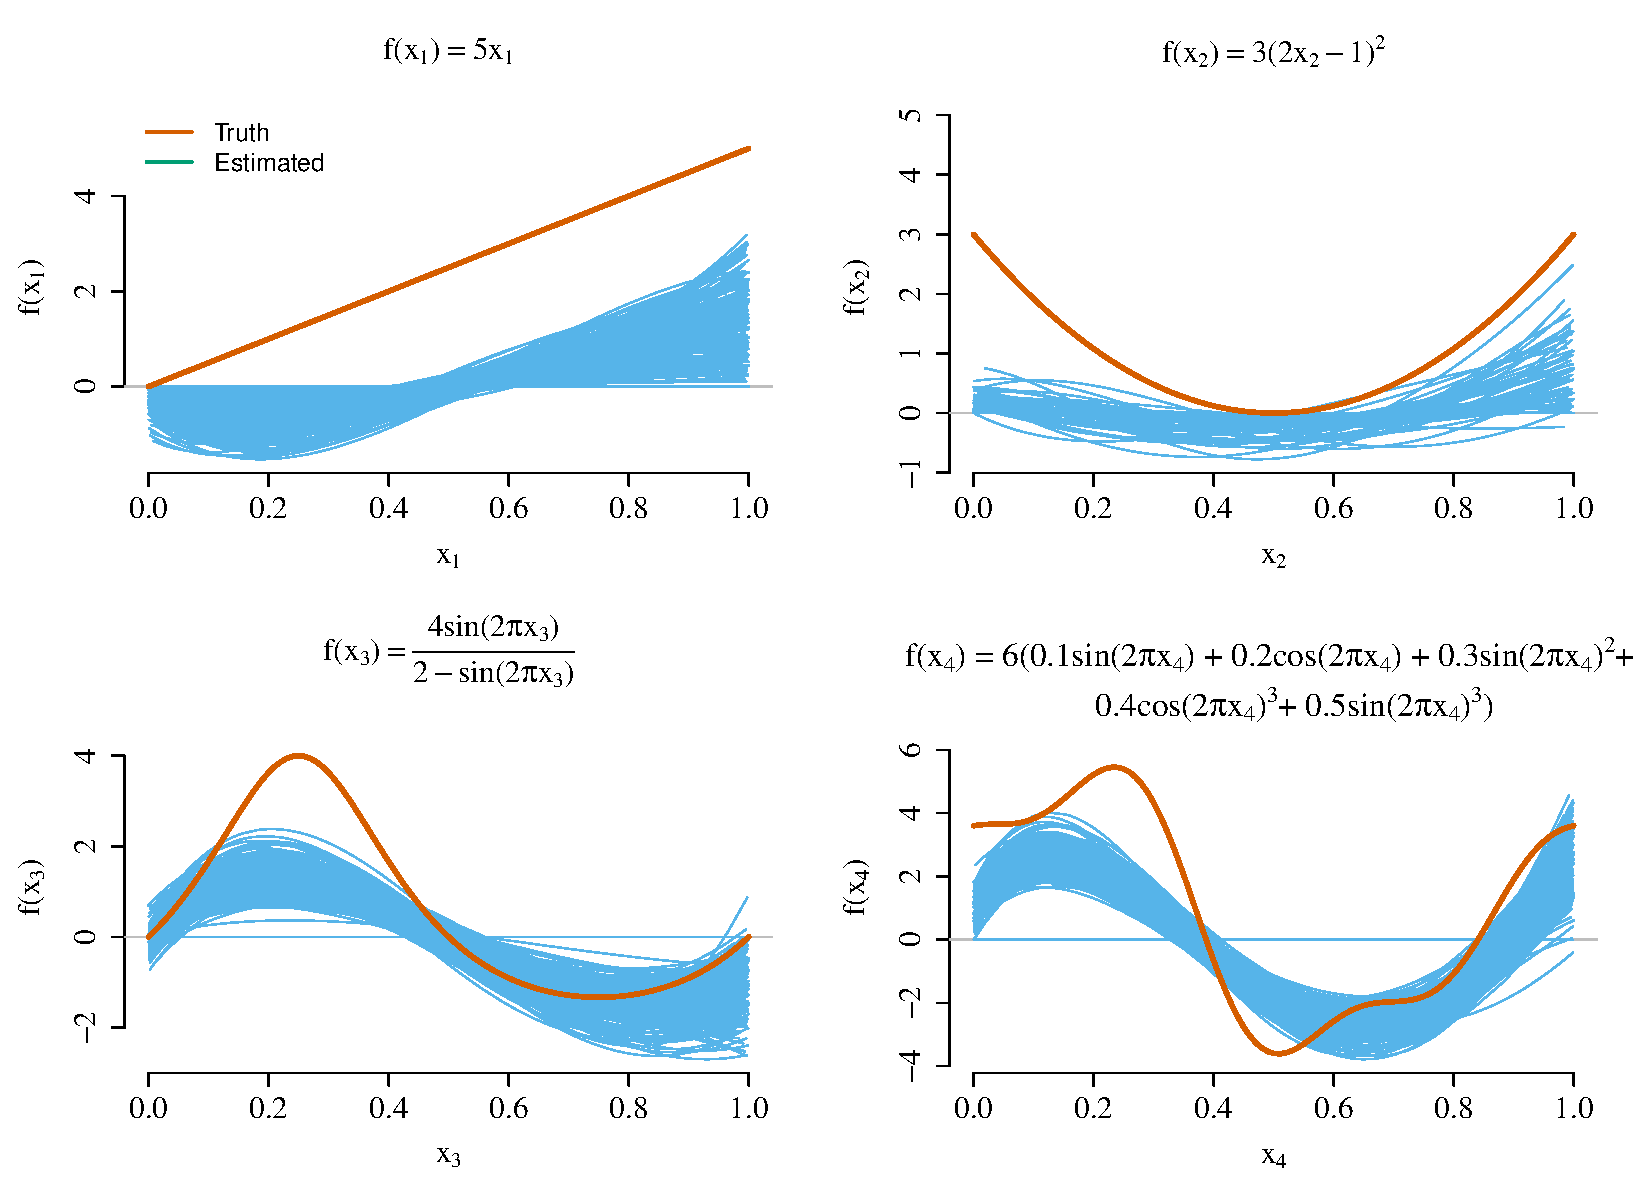
\includegraphics[scale=0.61]{/home/sahir/git_repositories/sail/my_sims/figures/sail_main_eff_paramIndex1_200sims.pdf}
	\caption{text}\label{fig:main_eff}
\end{figure}


\begin{figure}[H]
	\centering
	\subfloat{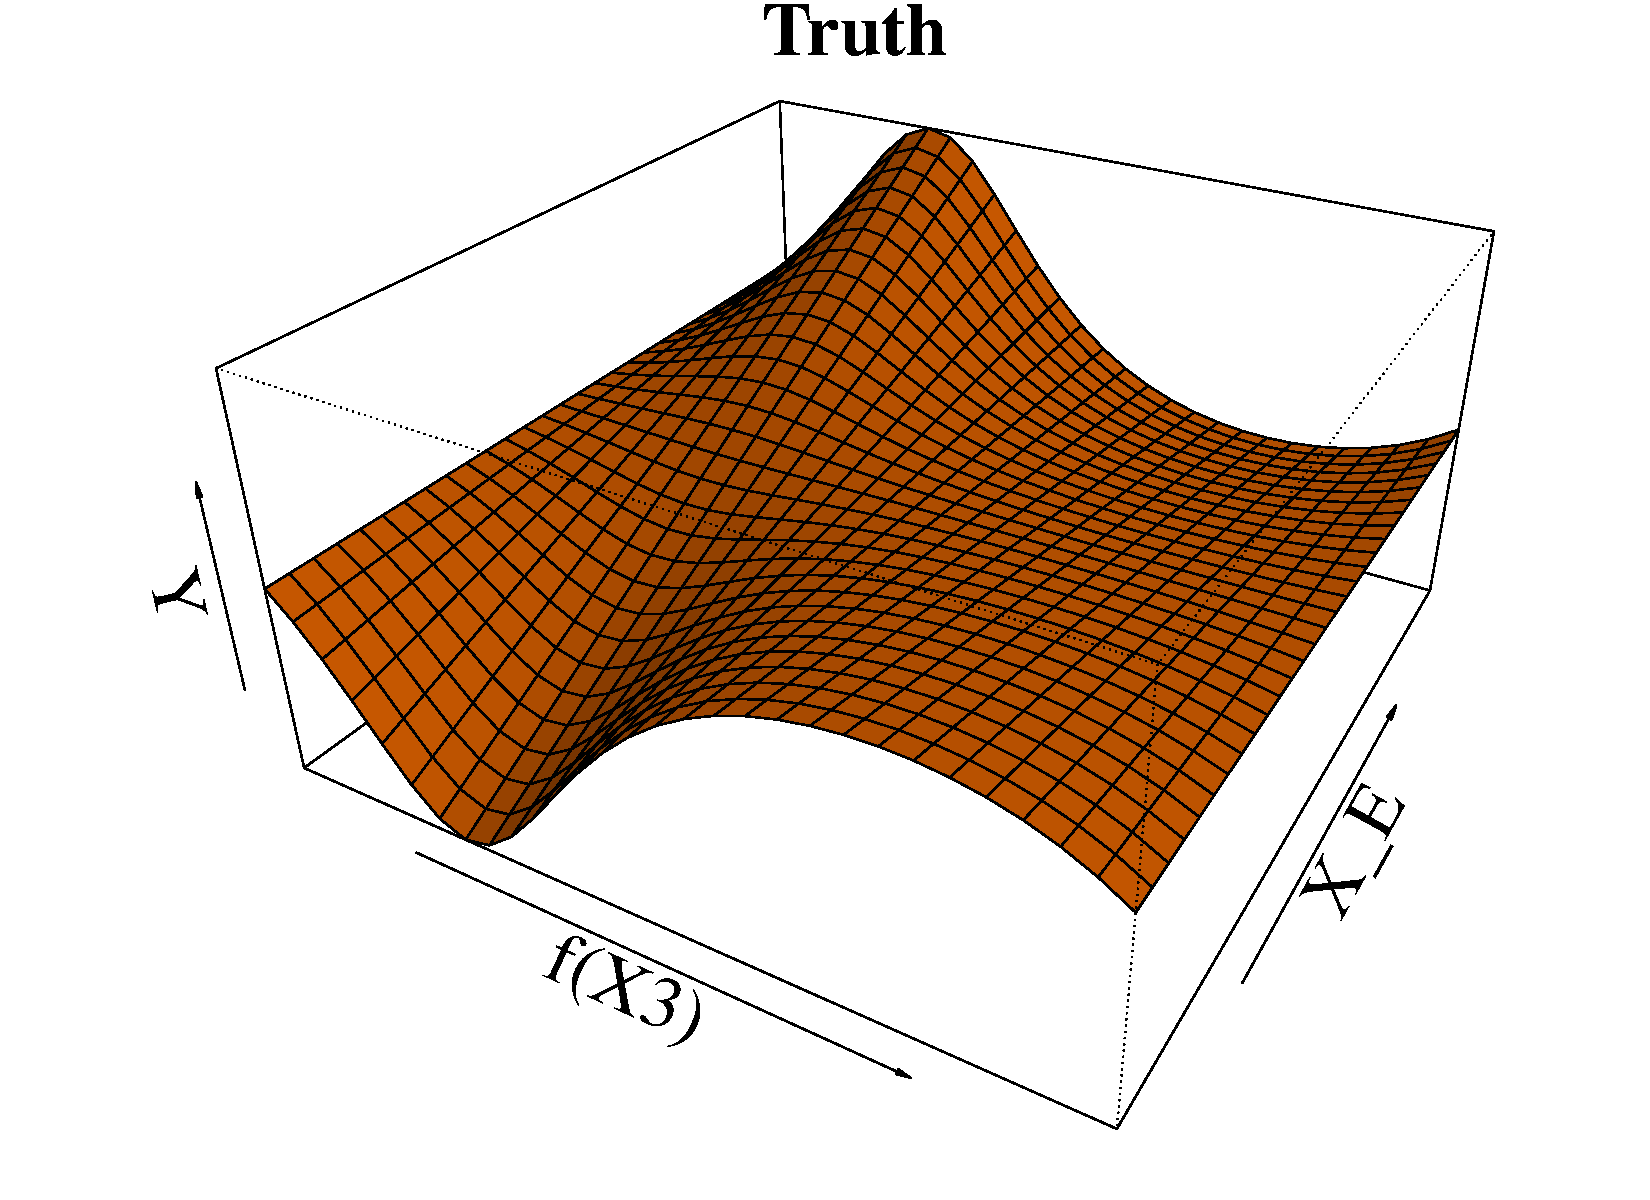
\includegraphics[width=0.50\linewidth]{/home/sahir/git_repositories/sail/my_sims/figures/sail_intertruth_X3_paramIndex1_200sims.pdf}}
	\subfloat{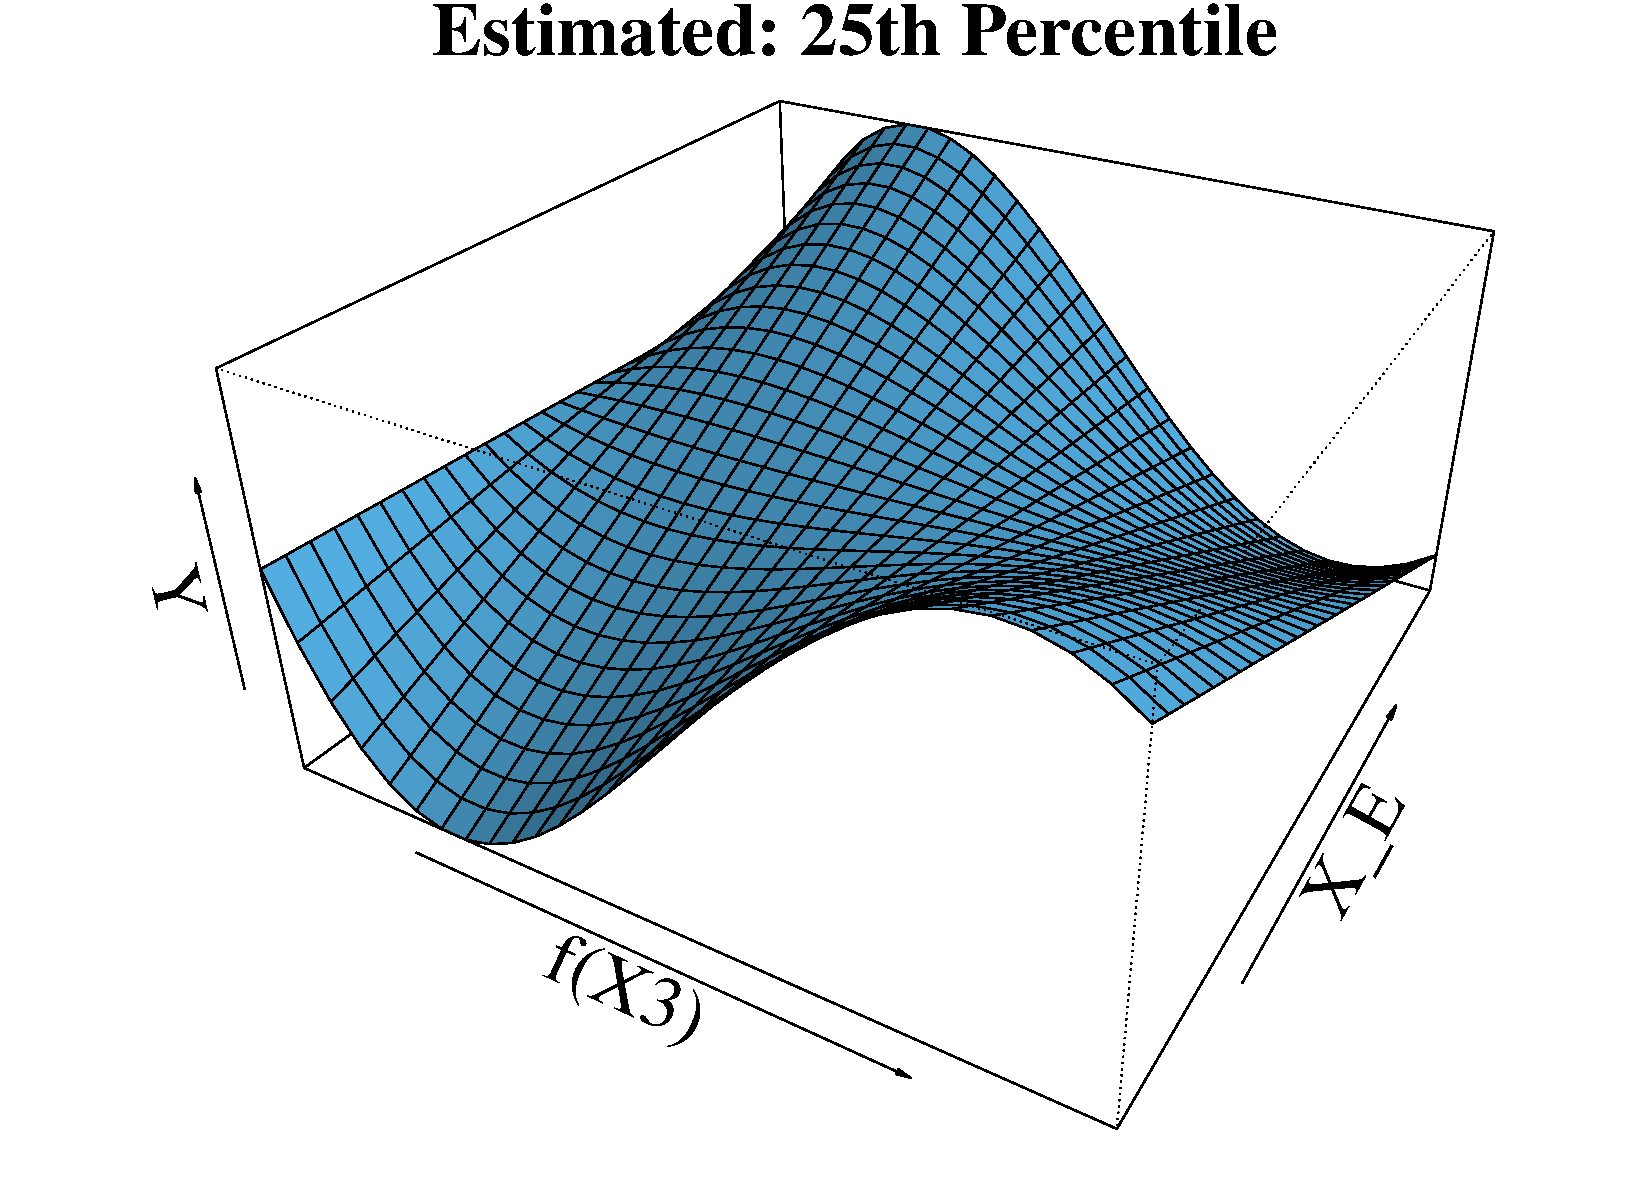
\includegraphics[width=0.50\linewidth]{/home/sahir/git_repositories/sail/my_sims/figures/sail_inter25_X3_paramIndex1_200sims.pdf}}\quad 
	\subfloat{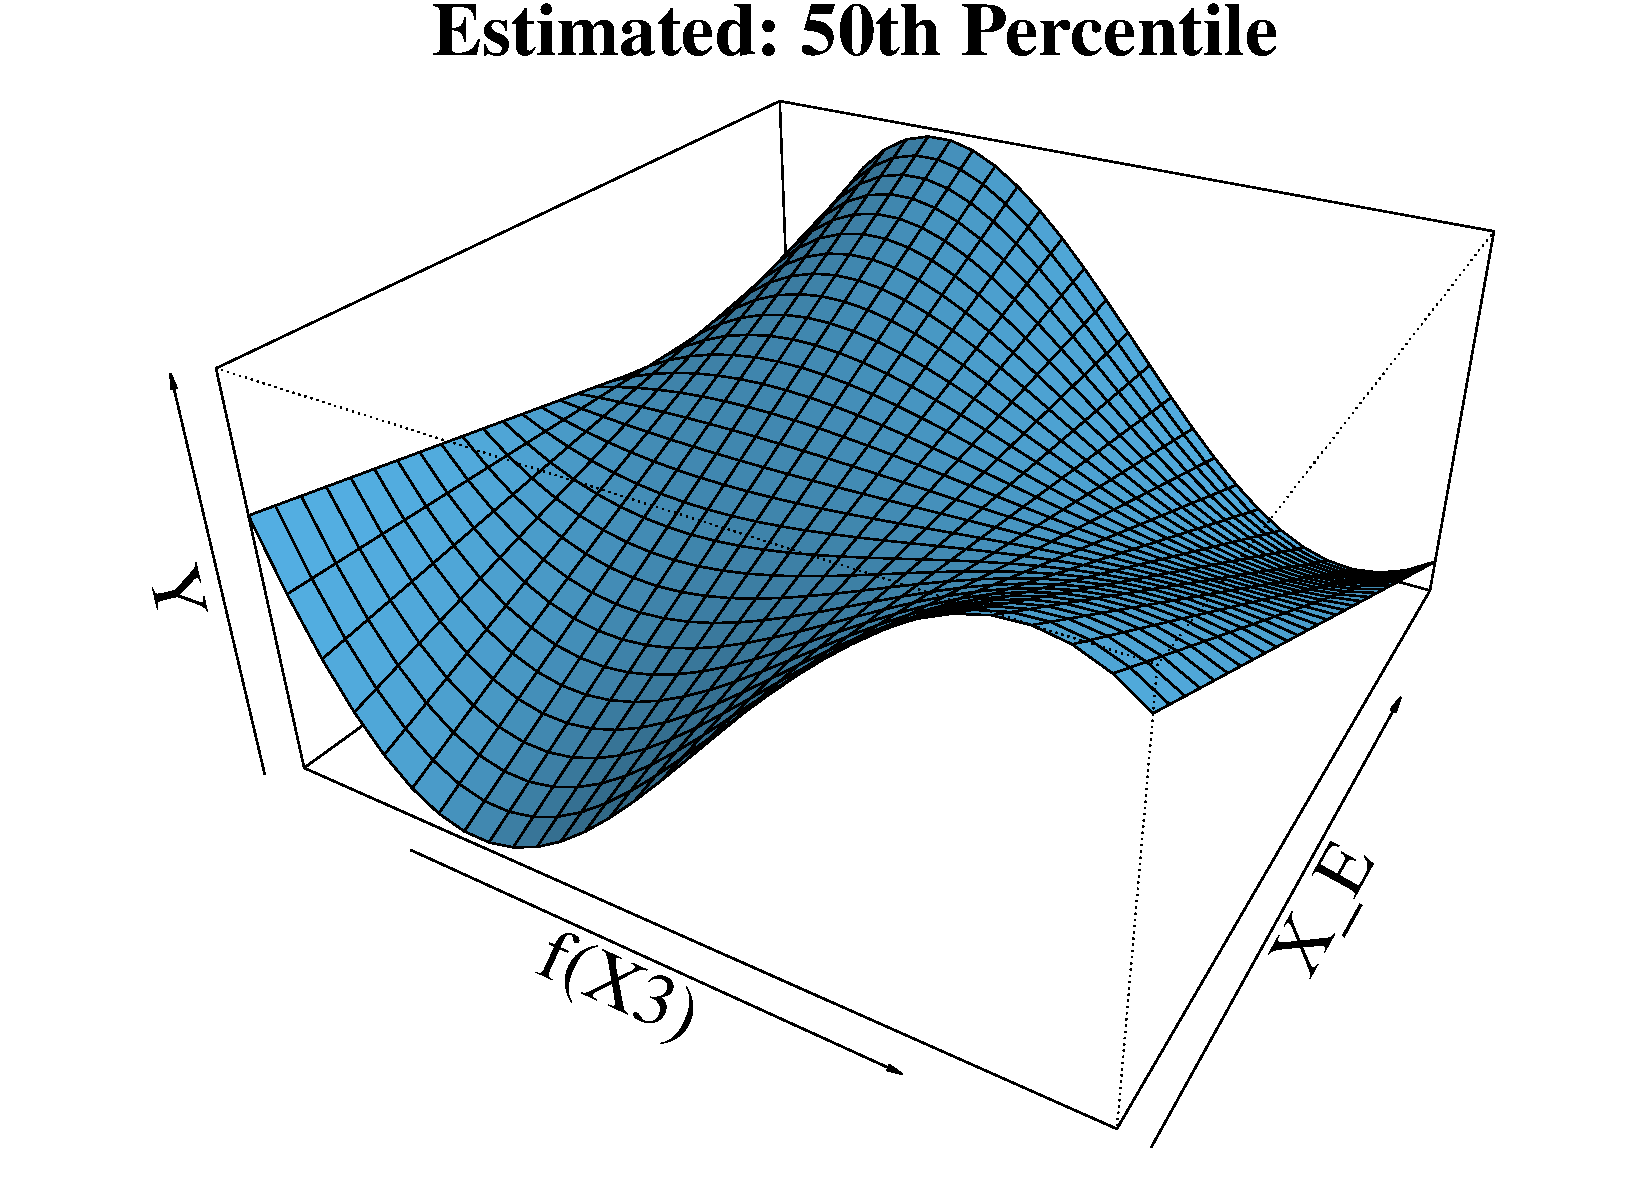
\includegraphics[width=0.50\linewidth]{/home/sahir/git_repositories/sail/my_sims/figures/sail_inter50_X3_paramIndex1_200sims.pdf}}
	\subfloat{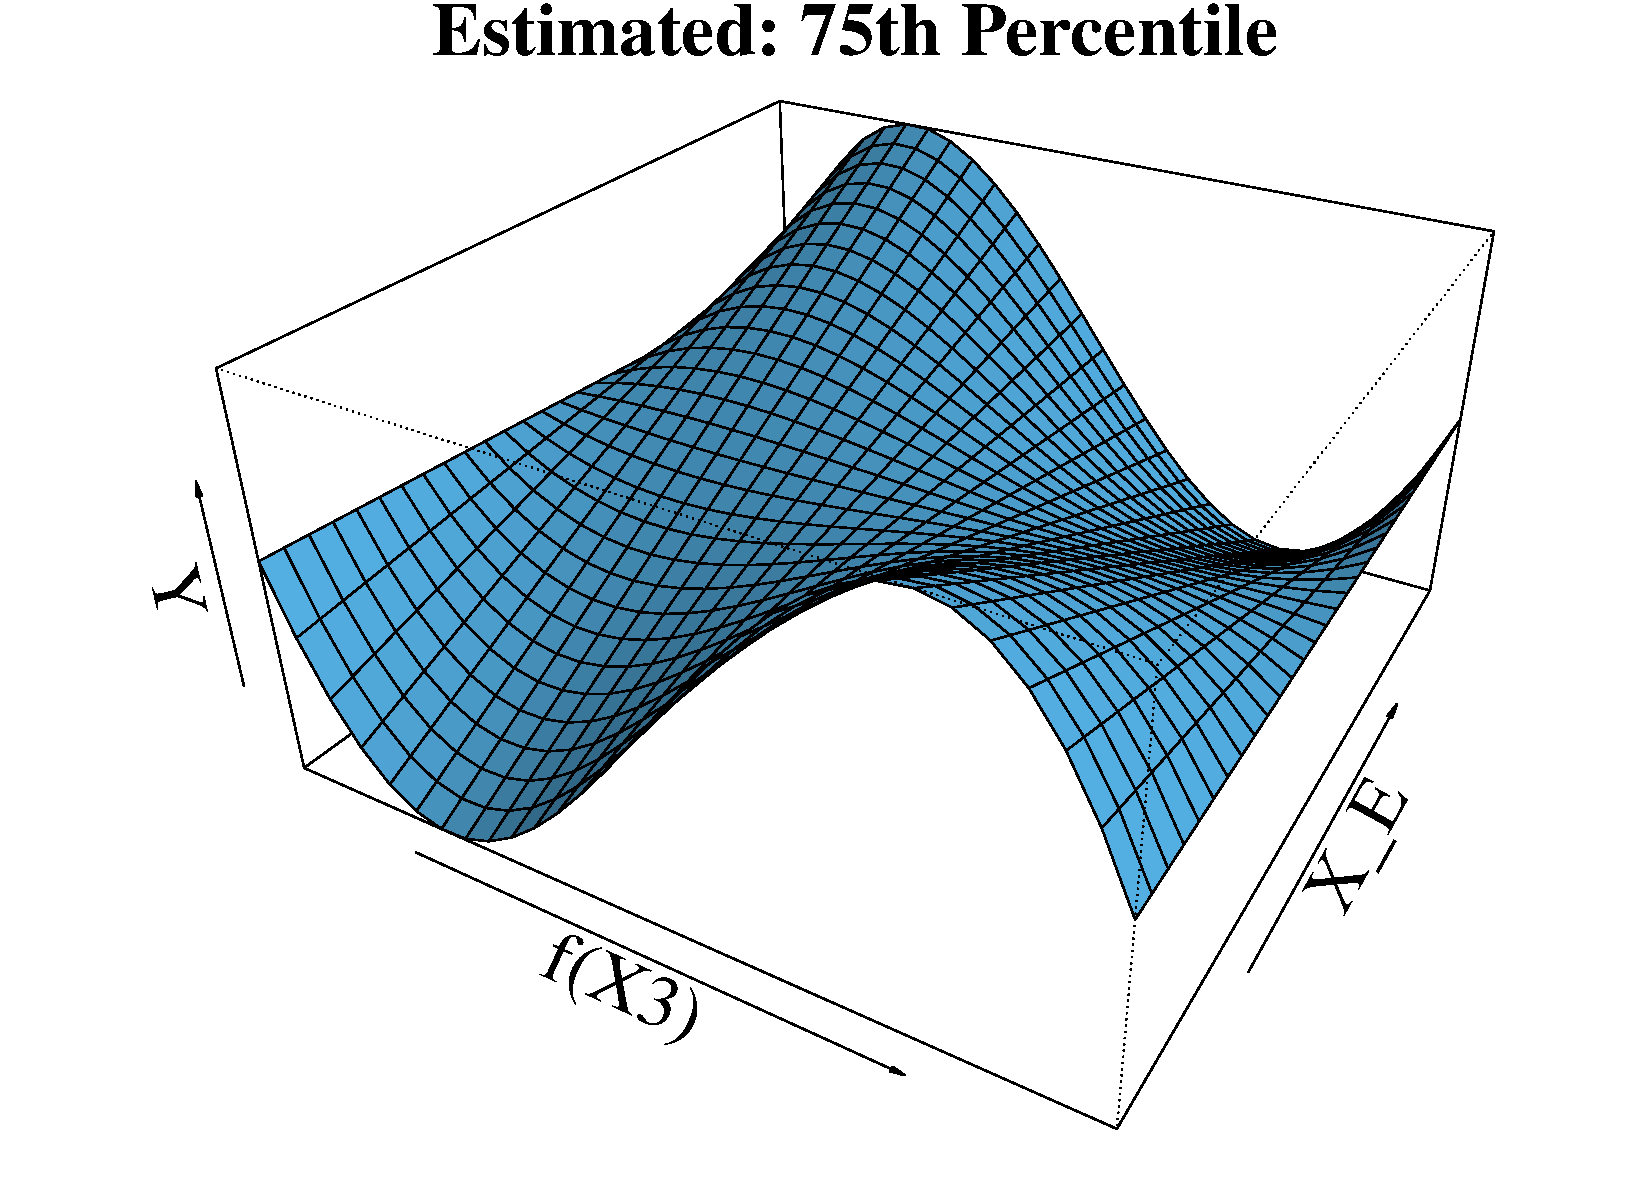
\includegraphics[width=0.50\linewidth]{/home/sahir/git_repositories/sail/my_sims/figures/sail_inter75_X3_paramIndex1_200sims.pdf}}
	\caption{True and estimated interaction effects for $E \cdot f(X_3)$ in simulation scenario 1a).}
	\label{fig:X3}
\end{figure}


\begin{figure}[H]
	\centering
	\subfloat{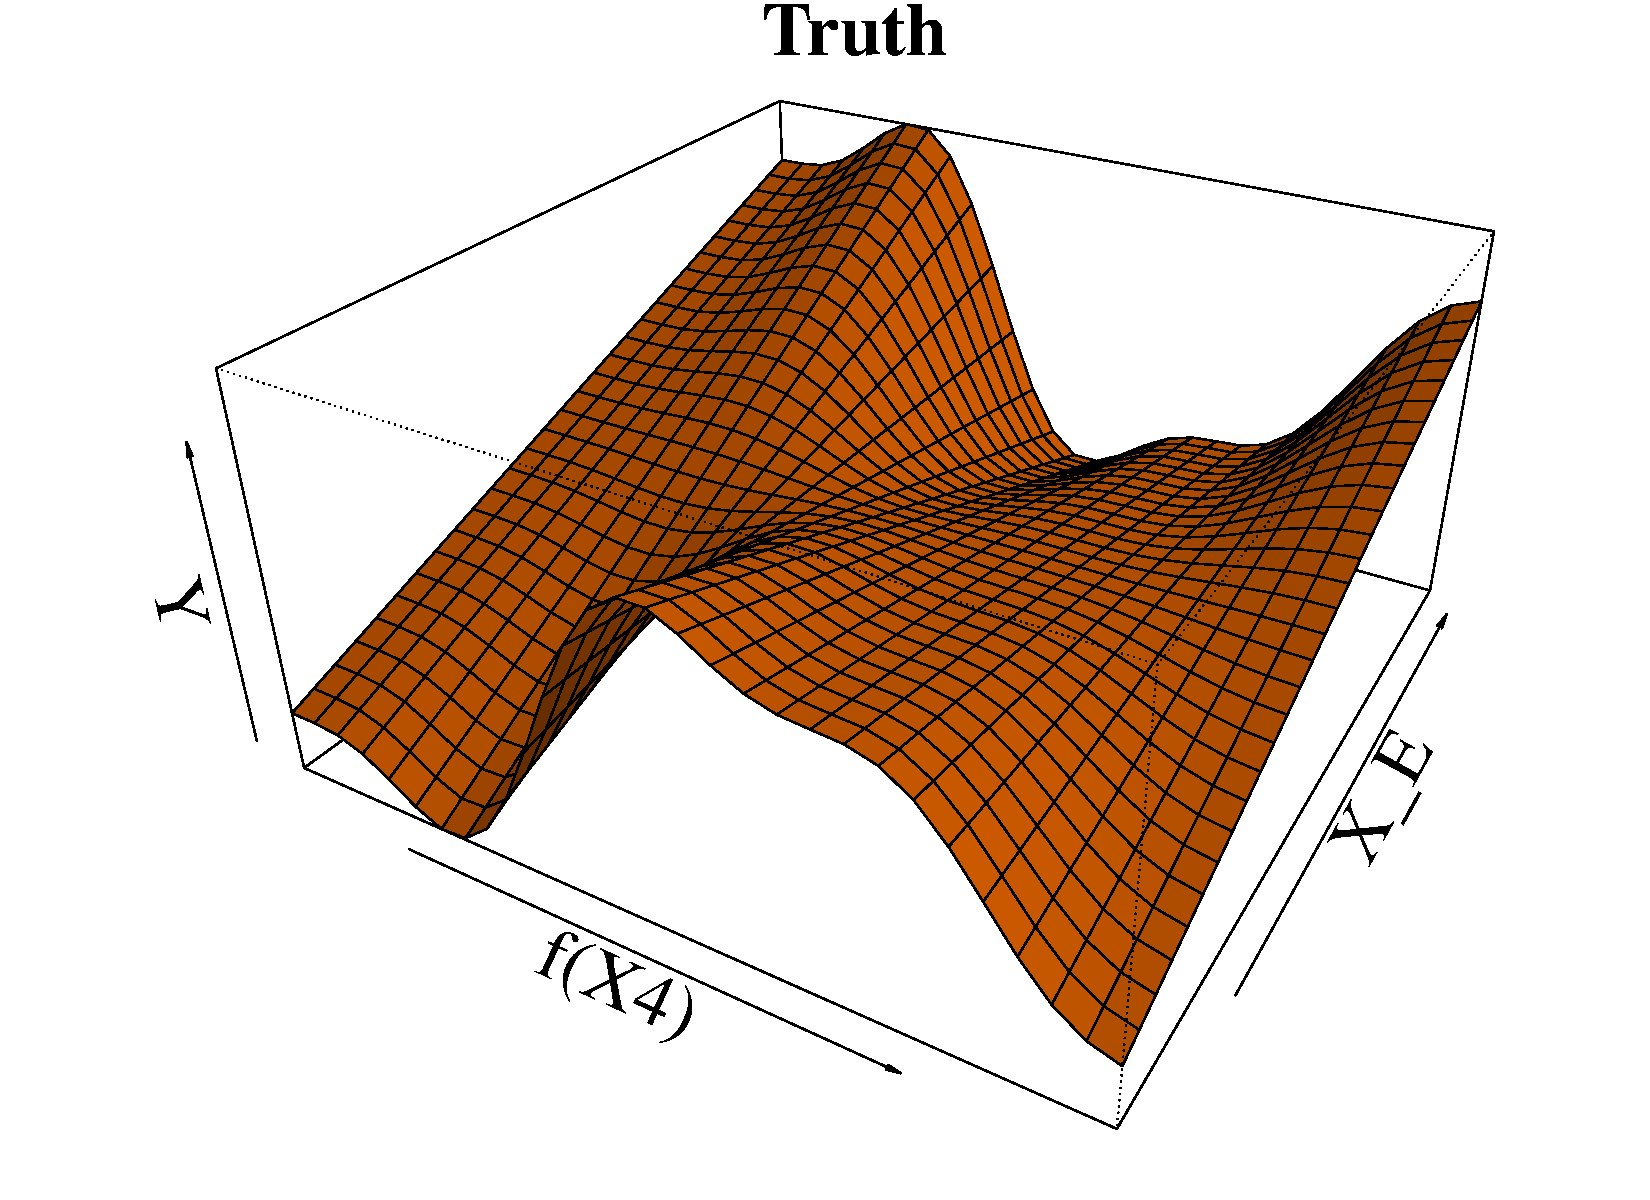
\includegraphics[width=0.50\linewidth]{/home/sahir/git_repositories/sail/my_sims/figures/sail_intertruth_X4_paramIndex1_200sims.pdf}}
	\subfloat{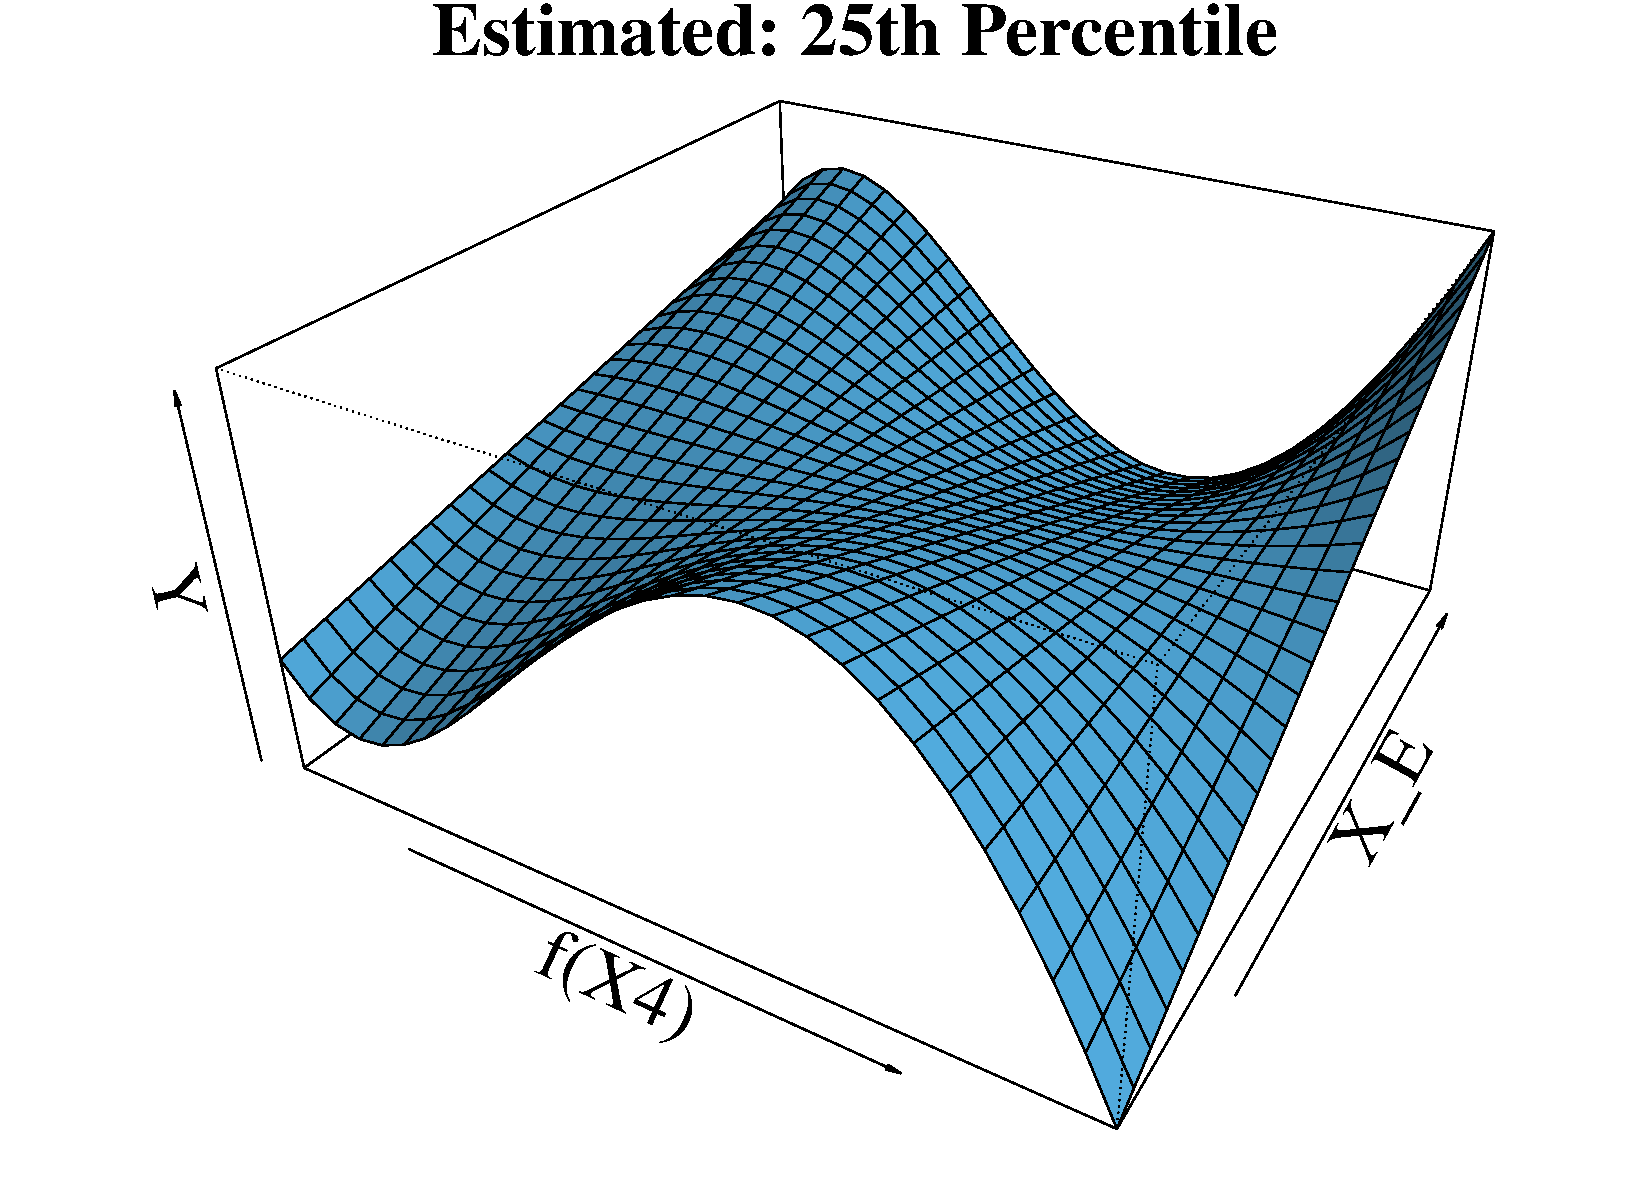
\includegraphics[width=0.50\linewidth]{/home/sahir/git_repositories/sail/my_sims/figures/sail_inter25_X4_paramIndex1_200sims.pdf}}\quad 
	\subfloat{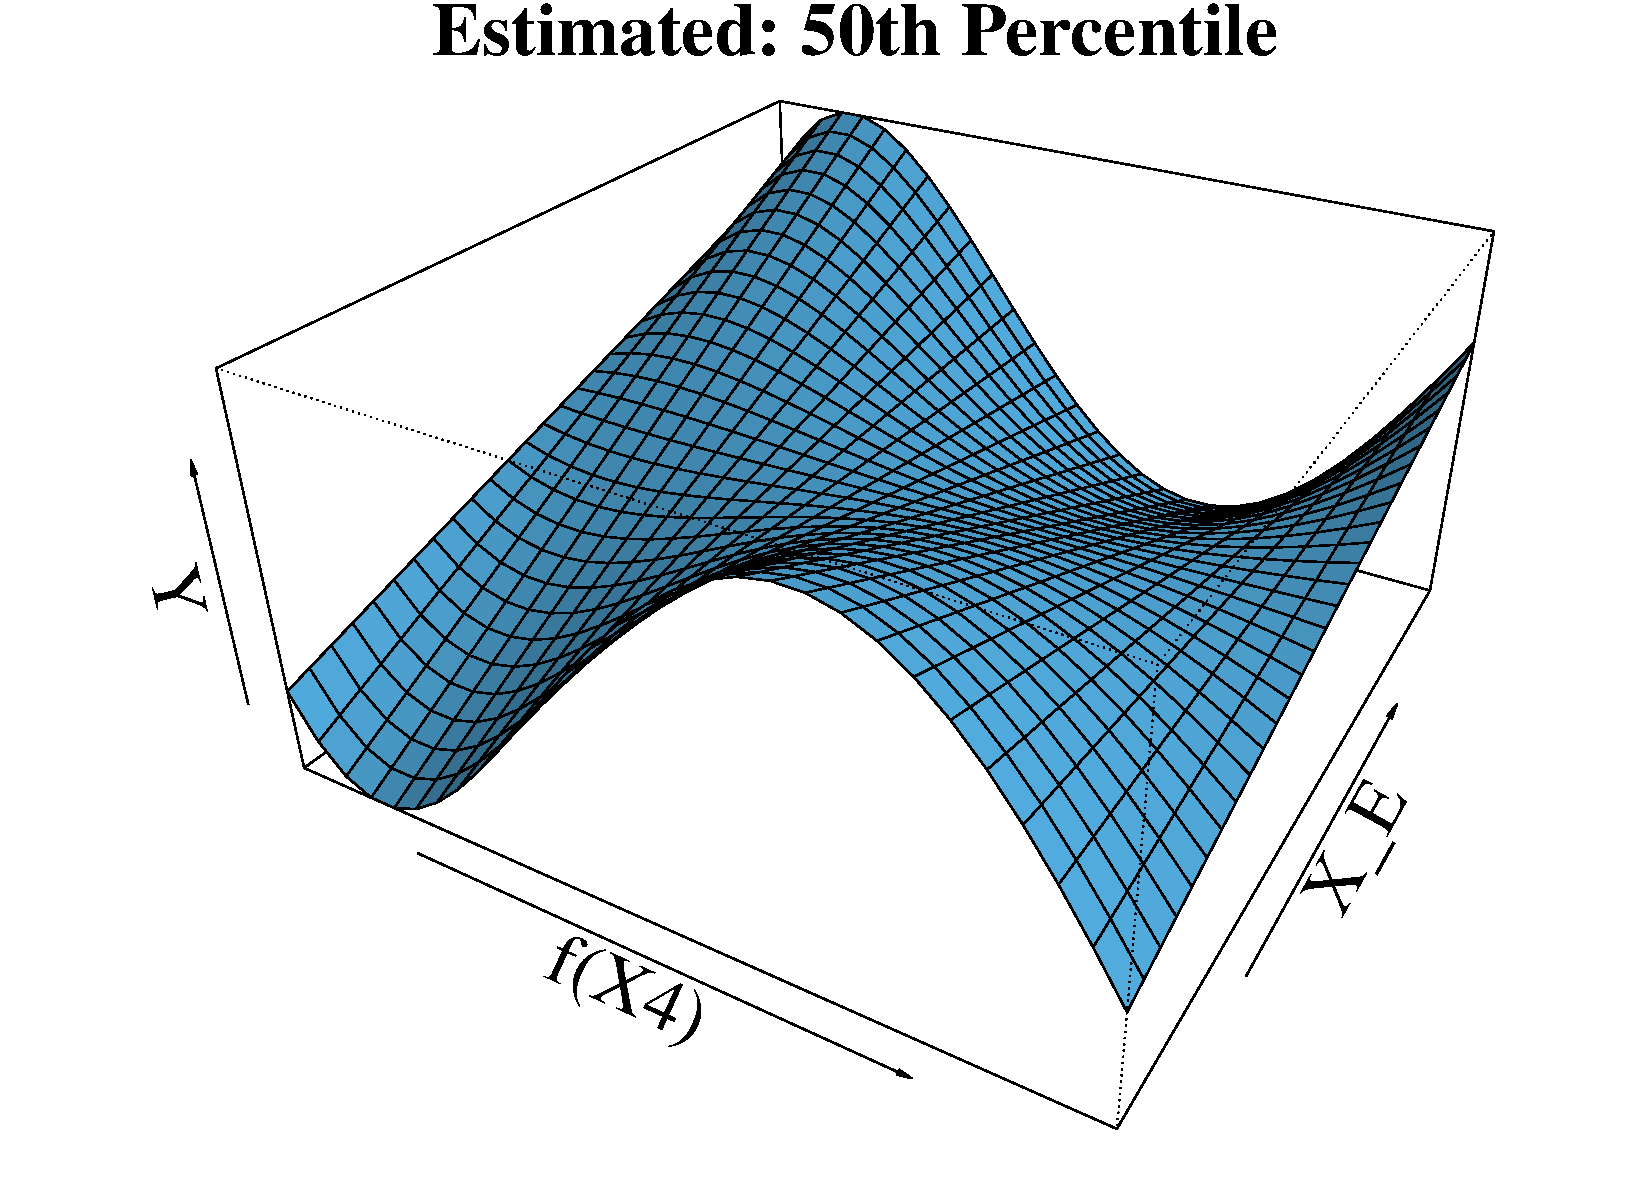
\includegraphics[width=0.50\linewidth]{/home/sahir/git_repositories/sail/my_sims/figures/sail_inter50_X4_paramIndex1_200sims.pdf}}
	\subfloat{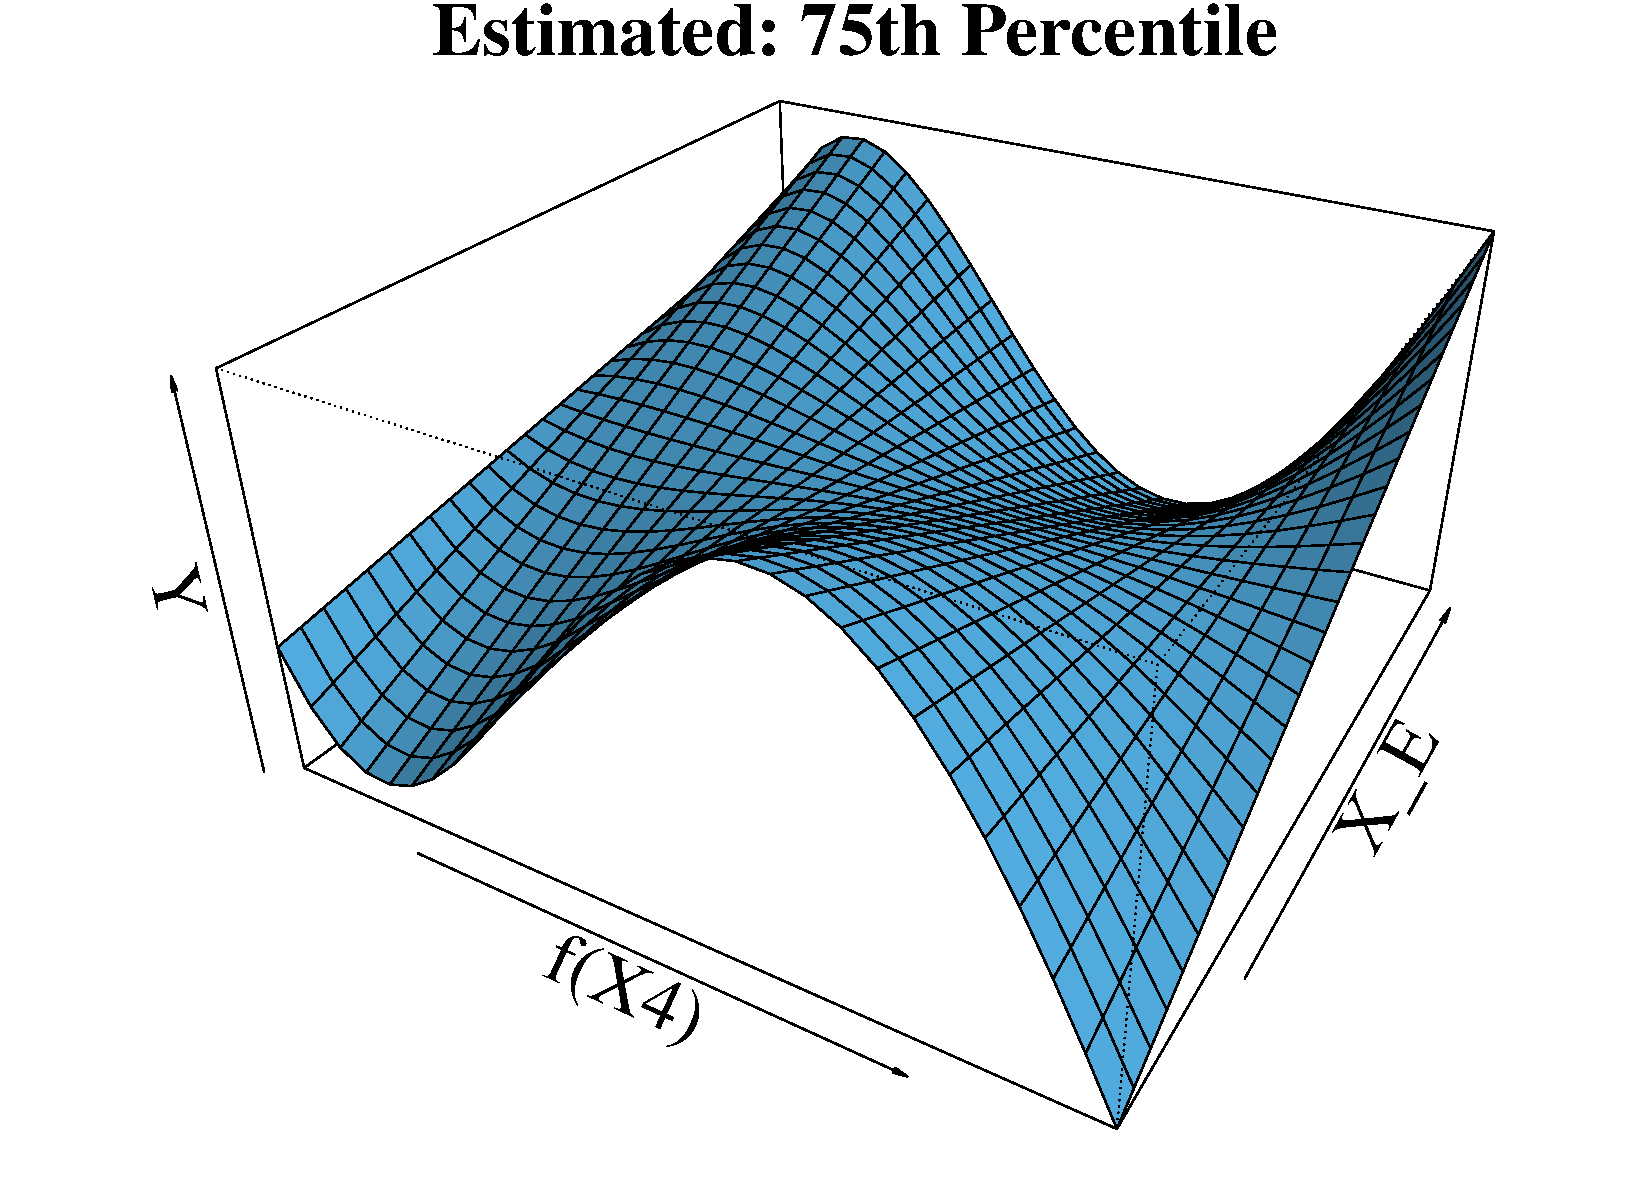
\includegraphics[width=0.50\linewidth]{/home/sahir/git_repositories/sail/my_sims/figures/sail_inter75_X4_paramIndex1_200sims.pdf}}
	\caption{True and estimated interaction effects for $E \cdot f(X_4)$ in simulation scenario 1a).}
	\label{fig:X4}
\end{figure}


\section{Real Data Application}



%\section{Application}

%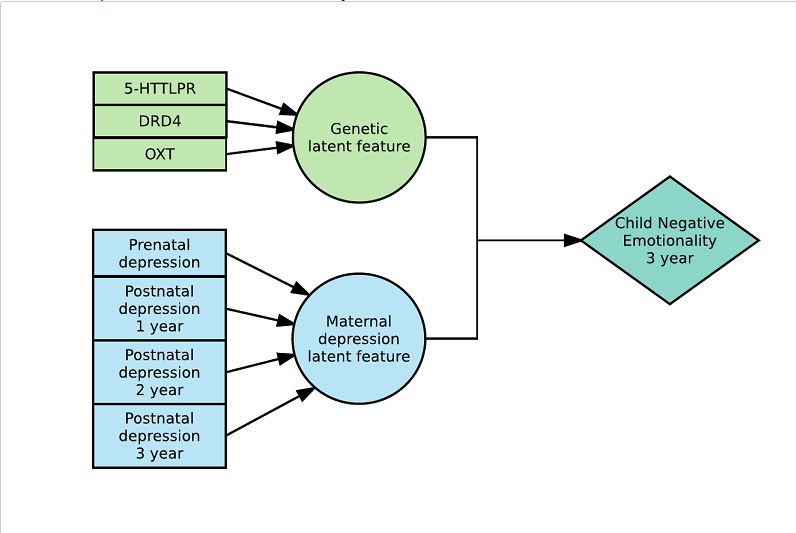
\includegraphics[scale=0.5]{l1}

%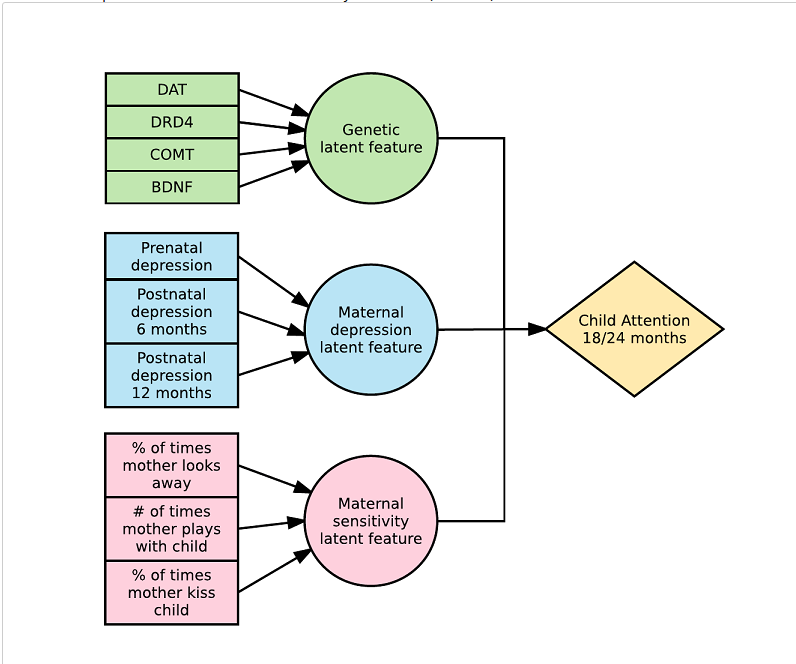
\includegraphics[scale=0.5]{l2}

\newpage
%\bibliographystyle{plainnat}
\bibliographystyle{abbrv}
%\addcontentsline{toc}{chapter}{References}
%\bibliographystyle{unsrtnat}
\bibliography{GEbib}


\end{document}


\subsection{Main Idea}
This manuscript addresses more traditional \textit{statistical} interaction models of the form 

\begin{equation}
	Y = X\beta_X + E \beta_E + X E \beta_{XE} + \varepsilon
\end{equation}

We propose to first filter out the noise variables (main effects only) using a method from the \textit{variable screening} literature, and then subsequently fit a penalized model, on the filtered set of variables, that enforces the strong heredity property, i.e., interaction terms can only be selected by the procedure if the main effects have been selected. 


\subsection{Introduction}

We consider a regression model for an outcome variable $Y=(y_1, \ldots, y_n)$ which follows an exponential family. Let $E=(e_1, \ldots, e_n)$ be the binary environment vector and $\bx = (X_{1}, \ldots, X_{p})$ be the matrix of high-dimensional data. Consider the regression model with main effects and their interactions with $E$:
\begin{align}
	g(\bmu)  = & \beta_0  + \underbrace{\beta_1 X_{1} + \cdots + \beta_p X_p + \beta_{E} E}_{\tm{main effects}} + \underbrace{\alpha_{1E} (X_1 E) + \cdots + \alpha_{pE} (X_p E)}_{\tm{interactions}} \label{eq:linpred1}
\end{align}
where $g(\cdot)$ is a known link function and $\bmu = \e\left[Y|\bx, E, \bbeta,\balpha\right]$. Our goal is to estimate the parameters \mbox{$\bbeta = \left(\beta_1, \beta_2, \ldots, \beta_p, \beta_E\right) \in \mathbb{R}^{p+1}$} and $\boldsymbol{\alpha} = \left(\alpha_{1E}, \ldots, \alpha_{pE}\right) \in \mathbb{R}^p$ and to improve prediction of $Y$. 

\subsection{Methods} \label{sec:varselect}

\subsubsection{Variable Screening}

Consider a binary response variable $Y=0,1$. A variable $X$ is independent of $Y$ \textit{iff} the conditional distributions of $X$ given $Y=0$ or $Y=1$ are identical. \citep{mai2012kolmogorov} proposed using the Kolmogorov-Smirnov (KS) test statistic
\begin{equation}
	\hat{K}_j = \sup_x \lvert \hat{F}_j(x|Y=1) - \hat{F}_j(x|Y=0)  \rvert   \label{eq:ks}
\end{equation}
to measure the dependence between $X_j$ and $Y$, where $\hat{F}_j$ is the empirical CDF of $X_j$. 

\citep{mai2015fused} then extended their method to a continuous response by essentially categorizing the response variable so that Eq.~\eqref{eq:ks} can be applied. They called this the Fused Kolmogorov filter.

\begin{figure}[H]
	\centering
	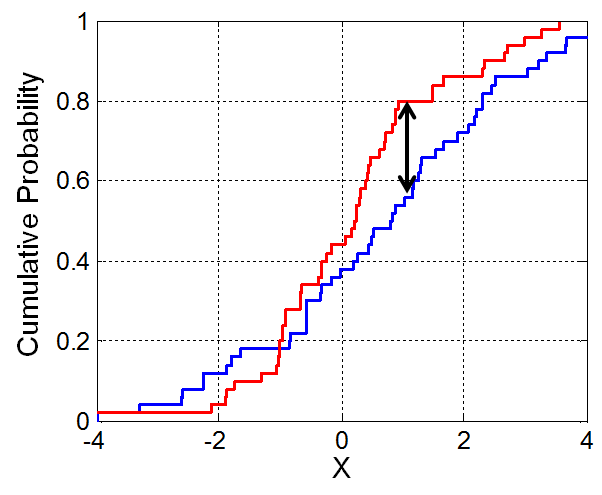
\includegraphics[scale=0.75]{./ks}
	\caption{Depiction of KS statistic}
	\label{fig:ks}
\end{figure}


\subsubsection{Strong Heredity Model}

We are interested in imposing the strong heredity principle~\citep{chipman1996bayesian}: 
\begin{equation}
	\hat{\alpha}_{jE} \neq 0 \qquad \Rightarrow \qquad \hat{\beta}_j \neq 0 \qquad \tm{and} \qquad \hat{\beta}_E \neq 0   \label{eq:heredity}
\end{equation}
In words, the interaction term will only have a non-zero estimate if its corresponding main effects are estimated to be non-zero. One benefit brought by hierarchy is that the number of measured variables can be reduced, referred to as practical sparsity~\citep{she2014group,bien2013lasso}. For example, a model involving $X_1, E, X_1 \cdot E$ is more parsimonious than a model involving $X_1, E, X_2 \cdot E$, because in the first model a researcher would only have to measure two variables compared to three in the second model. In order to address these issues, we propose to extend the model of Choi \textit{et al.}~\citep{choi2010variable} to simultaneously perform variable selection, estimation and impose the strong heredity principle in the context of high dimensional interactions with the environment (HD$\times E$). To do so, we follow Choi and reparametrize the coefficients for the interaction terms as $\alpha_{jE} = \gamma_{jE} \beta_j \beta_E$. Plugging this into~\eqref{eq:linpred1}:
\begin{align}
	g(\bmu)  = & \beta_0  + \beta_1 \widetilde{X}_{1} + \cdots + \beta_q \widetilde{X}_q + \beta_{E} E + \gamma_{1E}\beta_1 \beta_E (\widetilde{X}_1 E) + \cdots + \gamma_{qE}\beta_q \beta_E (\widetilde{X}_q E)    \label{eq:linpred2}
\end{align}
where $\widetilde{\bx} = (\widetilde{X}_1, \ldots, \widetilde{X}_q)$ are the cluster representatives derived in phase 2 and $q <p$. This reparametrization directly enforces the strong heredity principle (Eq.~\eqref{eq:heredity}), i.e., if either main effect estimates are 0, then $\hat{\alpha}_{jE}$ will be zero and a non-zero interaction coefficient implies non-zero $\hat{\beta}_j$ and $\hat{\beta}_E$. To perform variable selection in this new parametrization, we follow Choi \textit{et al.}~\citep{choi2010variable} and penalize $\bs{\gamma} = \left(\gamma_{1E}, \ldots, \gamma_{pE}\right)$, leading to the following penalized least squares criterion:
\begin{equation}
	\argmin_{\beta_0, \bbeta, \bs{\gamma} }  \frac{1}{2} \norm{Y - g(\bmu)}^2 + \lambda_\beta \left(w_1 \beta_1 + \cdots + w_q \beta_q + w_E \beta_E   \right) + \lambda_\gamma  \left( w_{1E} \gamma_{1E} + \cdots + w_{qE}\gamma_{qE}         \right) \label{eq:lassolikelihood2}
\end{equation} 
where $g(\bmu)$ is from~\eqref{eq:linpred2}, $\lambda_\beta$ and $\lambda_\gamma$ are tuning parameters and $\mb{w} = \left(w_{1}, \ldots, w_q, w_{1E}, \ldots, w_{qE}\right)$ are prespecified adaptive weights. The $\lambda_\beta$ tuning parameter controls the amount of shrinkage applied to the main effects, while $\lambda_\gamma$ controls the interaction estimates and allows for the possibility of excluding the interaction term from the model even if the corresponding main effects are non-zero. The adaptive weights serve as a way of allowing parameters to be penalized differently. Furthermore, adaptive weighting~\citep{zou2006adaptive} has been shown to construct oracle procedures~\citep{fan2001variable}, i.e., asymptotically, it performs as well as if the true model were given in advance. The oracle property is achieved when the weights are a function of any root-$n$ consistent estimator of the true parameters e.g. maximum likelihood (MLE) or ridge regression estimates. It can be shown that the procedure in~\eqref{eq:lassolikelihood2} asymptotically possesses the oracle property~\citep{choi2010variable}, even when the number of parameters tends to $\infty$ as the sample size increases, if the weights are chosen such that
\begin{equation}
	w_j = \left | \frac{1}{\hat{\beta}_j} \right|, \quad w_{jE} = \left | \frac{\hat{\beta}_j \hat{\beta}_E}{\hat{\alpha}_{jE}} \right| \quad \tm{ for }j=1, \ldots, q   \label{eq:weights}
\end{equation}
where $\hat{\beta}_j$ and $\hat{\alpha}_{j}$ are the MLEs, \textit{using the transformed variables}, from~\eqref{eq:linpred1} or the ridge regression estimates when $q > n$. The rationale behind the data-dependent $\hat{\bs{w}}$ is that as the sample size grows, the weights for the truly zero predictors go to $\infty$ (which translates to a large penalty), whereas the weights for the truly non-zero predictors converge to a finite constant~\citep{zou2006adaptive}. 

There have been several more recent proposals for modeling interactions with the strong heredity constraint in the variable selection via penalization literature including Composite Absolute Penalties (CAP)~\citep{zhao2009composite}, Variable selection using Adaptive Nonlinear Interaction Structures in High dimensions (VANISH)~\citep{radchenko2010variable}, Strong Hierarchical Lasso (hierNet)~\citep{bien2013lasso}, Group-Lasso Interaction Network (glinternet)~\citep{lim2014learning}, Group Regularized Estimation under Structural Hierarchy (GRESH)~\citep{she2014group} and a Framework for Modeling Interactions with a Convex Penalty (FAMILY)~\citep{haris2014convex}. While each method has their own merit, including that they are all convex optimization problems, they all contain complex penalty functions which are hard to interpret and lead to computationally expensive fitting algorithms. On the other hand, the objective function in~\eqref{eq:lassolikelihood2} can be solved using an iterative approach (by first fixing $\bbeta$ and then $\balpha$) which simplifies to a LASSO type problem; one that has been extensively studied, is well understood and can be solved efficiently using existing software (e.g. \texttt{glmnet}~\citep{friedman2010regularization}). A limitation of this approach is that the optimization problem is non-convex, arising from the reparametrization of $\balpha$ as a product of optimization variables $(\bbeta, \bs{\gamma})$, and hence convergence to the global minimum is not guaranteed~\citep{choi2010variable}. 


\subsection{Simulation Study}


\subsection{Real-Data Example}


\subsection{Novelty and Contributions}

The fused Kolmogorov filter with the strong heredity model has not been previously investigated. 

To our knowledge, strong hierarchies have never previously been used in HD interaction analysis in genomics or brain imaging studies. Furthermore, the specific choices of weights proposed here, i.e., based on the transformed variables from phase 2, have not been previously used. Choi \textit{et al.}~\citep{choi2010variable} estimated their weights simultaneously, but this would not be feasible in HD data. The adaptation to interactions with one key $E$ variable is specific to our situation.

References~\cite{radchenko2010variable,zhao2009composite,she2014group,choi2010variable} (which includes the one that our proposal is based on) failed to provide any code or software for their method. Not only does this prevent applied researchers from using these advanced techniques, it also hinders statisticians from comparing the performance of their newly developed method against existing approaches. Indeed, a survey of the citations of these papers reveals that they are seldom used in practice or as a comparison method in theoretical papers, and only cited in literature review paragraphs. Three approaches that have provided \texttt{R} packages (\texttt{hierNet}~\citep{bien2013lasso}, \texttt{glinternet}~\citep{lim2014learning} and \texttt{FAMILY}~\citep{haris2014convex}) are only suited for all pairwise interactions of the design matrix (the theory in \texttt{FAMILY} does not impose such a restriction but the software returns an error when we input a 1 column environment variable) and are not designed for the HD$\times E$ interactions that are the focus of this thesis. Therefore, a novel aspect of this thesis will be the development of a procedure for $\tm{HD}\times E$ interactions which simultaneously performs variable selection and estimation, follows the strong heredity principle and is an oracle procedure, as well as its implementation into a computationally fast open source \texttt{R} package.
